\documentclass[11pt]{article}
\usepackage[english]{babel}
\usepackage{bm}       % Required for bold math symbols
\usepackage{comment}
\usepackage{booktabs}
\usepackage{subcaption}
\usepackage{siunitx}
\usepackage{enumitem}
\usepackage[a4paper,top=2cm,bottom=2cm,left=2cm,right=2cm]{geometry}
\usepackage{amsmath}
\usepackage{graphicx}
\usepackage[colorlinks=true, allcolors=blue]{hyperref}
\captionsetup{font=footnotesize} % can also use \scriptsize

% Adjust section title font sizes
\usepackage{titlesec}
%\titleformat*{\section}{\normalsize\bfseries}
%\titleformat*{\subsection}{\small\bfseries}
%\titleformat*{\subsubsection}{\small\bfseries}

\titlespacing*{\section}{0pt}{1ex}{0.5ex}
\titlespacing*{\subsection}{0pt}{1ex}{0.5ex}
\titlespacing*{\subsubsection}{0pt}{0.5ex}{0.5ex}

% Reduce space above and below figures
\setlength{\abovecaptionskip}{3pt}
\setlength{\belowcaptionskip}{0pt}
\setlength{\intextsep}{5pt} % Adjust this value as needed

\title{OP34: The Zeeman effect}
\author{Andrei-Nicolae Taropa}

\begin{document}
\maketitle

%-------------------------------------------------------------------

\begin{abstract}
The Zeeman effect predicts splitting of atomic energy levels proportional to an applied magnetic field. Here we use a Fabry-Perot interferometer to measure changes caused by an external magnetic field in the fine structure of cadmium and mercury, where the fine structure is determined by the spin orbit interaction. DO I NEED TO SPECIFY WHAT THE FINE STRUCTURE IS? The experiment verified the theoretical prediction by checking the effect of every quantum number on the Landé g factor and consequently on the individual energy level. Additionally, the experiment investigated the type of polarised light emitted, identified the handedness of the circularly polarised light, therefore confirming the selection rules that arise from a quantum-mechanical treatment of the phenomenon. The experimental results were in agreement with the theory and there were no higher order perturbations, unaccounted for by the Zeeman effect, observable with the resolution achieved by this setup. 
\end{abstract}

%-------------------------------------------------------------------

\section{Introduction}
Transitions of the electrons between the different atomic energy levels create the specific atomic spectra. When introduced in a magnetic field, some of the spectral lines split into multiple components. 
% need to verify this is correct
The splitting of quantum mechanical energy levels in a weak magnetic field is best described by the Zeeman effect. 
In the semi-classical Bohr model for the atom, the interaction of the magnetic moment $\mu_B$ caused by the orbital motion of the electron with the external field $B$ leads to a simple energy level splitting $\pm \mu_B B$ (the \emph{normal} Zeeman effect). 
However, this model does not include the spin magnetic moment and therefore it only correctly predicts energy level splitting when the total spin is $0$. A quantum-mechanical model of an atom incorporating the spin magnetic moment $m_s$ predicts an energy split of $m_s g_L \mu_B B$, where $g_L$ is the Landé g factor. Historically this phenomenon was called the \emph{anomalous} Zeeman effect, because the spin interaction can not be explained classically. The anomalous Zeeman effect predicts an energy dependence on the quantum numbers $j$, $l$, and $s$, for total angular momentum, orbital angular momentum and spin respectively, as verified in this report.

Our experiments observed the normal Zeeman effect using the red (644 nm) transition line of a cadmium lamp. The anomalous Zeeman effect was investigated in the cadmium green (509  nm) transition line. A mercury lamp was utilised to observe the green (546 nm) and the blue (435 nm) transition lines. The lines were observed in two configurations: perpendicular to the magnetic field (both the $\pi$ and $\sigma$ polarisation is visible) and along the field lines (only $\sigma$ polarisation is visible). These measurements can fully verify the dependence of the splitting on spin, orbital angular momentum and total angular momentum. 

In this paper we first discuss the theory behind the Zeeman effect (section \ref{sec: theory}), the experimental setup (section \ref{sec: aparatus}) and the methods used to measure the energy level splitting (section \ref{sec: measuremet}). We include a detailed discussion of the measurement uncertainties and assumptions made during the data analysis (section \ref{sec: err}). Section \ref{sec: results} presents the results we obtained and how they are in agreement with the established theory. We end with the a summary of our results and future applications (section \ref{sec: conclusion}). 

%-------------------------------------------------------------------

\section{Theory and Methods}
\subsection{Energy levels and allowed transitions} \label{sec: theory}
One can find energy levels of an atom by considering the following Hamiltonian: 
\begin{equation}
    H = H_{CF} + H_{RE} + H_{SO} + H_{ZE} \label{eq: atomic ham}
\end{equation}
where $H_{CF}$ is the interaction with the central field, giving the gross structure of the energy levels, $H_{RE}$ is the residual electrostatic perturbation, $H_{SO}$ is the spin-orbit interaction perturbation and $H_{ZE}$ is the interaction with an external magnetic field. In the weak field limit $H_{ZE} \ll H_{SO} \ll H_{RE}$ we can treat the Zeeman interaction $H_{ZE}$ as a perturbation to the fine-structure levels that arise from L-S coupling \cite{Binney_Skinner_2015}. The energy of the $H_{ZE}$ interaction comes from the precessional motion of the orbital and spin magnetic moments around the external field: 

\begin{equation}
    H_{ZE} = \mu_B B \cdot (g_L L + g_S S) \label{eq: Hze}
\end{equation}
where $g_L = 1$ and $g_S = 2$ are the g-factors for the orbit and spin respectively. $|n l s j m_L >$ is the natural basis for the perturbation because it diagonalises the Hamiltonian $H_{ZE}$ \cite{foot2005atomic}. This is because in order to calculate the energy perturbation of the energy level $\Delta E_{ZE}$ one needs to take the time average of the operators in equation \eqref{eq: Hze}. $L \cdot B$ and $S \cdot B$ are not constants of motion, but $J \cdot B$ is. We consider projections of $L$ and $S$ along $J$: 
\begin{equation}
    H_{ZE} = \mu_B B \cdot J(g_L \frac{|L \cdot J|}{|J|^2} + 
    g_S \frac{|S \cdot J|}{|J|^2}) \label{eq: Hze J}
\end{equation}
We cast the equation into the form \eqref{eq: E lvl}, where the Landé g factor is \eqref{eq: gl}: 
\begin{equation}
    \Delta E_{ZE} = m_J g_L \mu_B B \label{eq: E lvl}
\end{equation}
The splitting is a function of the j, l, and s quantum numbers: 
\begin{equation}
    g_L = 1 + \frac{j(j+1)-l(l+1) +s(s+1)}{j(j+1)} \label{eq: gl}
\end{equation}

\begin{figure}[h!]
    \centering
    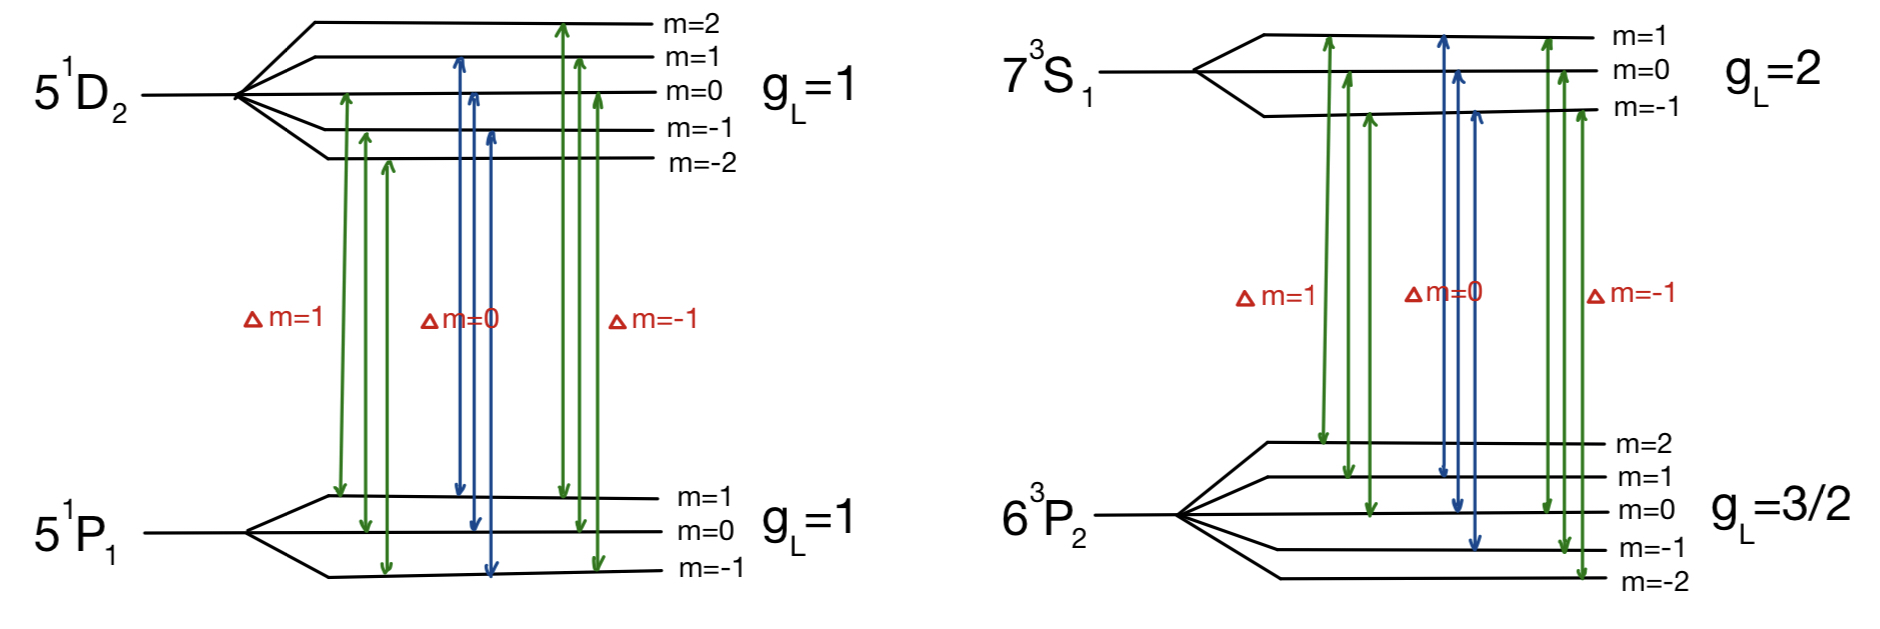
\includegraphics[width=\linewidth]{Energy levels.png}
    \captionsetup{justification=centering}
    \caption{Schematic diagram of the Zeeman splitting. 
    \textbf{Left side:} normal Zeeman effect in the Cadmium red line. The Landé g factors $g_L = 1$ for Cadmium, thus the line splits into 3 components. 
    \textbf{Right side:} anomalous Zeeman effect in the Mercury green line. The splitting is identical to the Cadmium green line splitting. The Landé g factors $g_L$ for Mercury are $2$ and $3/2$, thus the line splits into 9 components. }
    \label{fig: energy levels}
\end{figure}
The energy difference $E$ between the two levels of the transition can be written neatly in the form of equation \eqref{eq: E}, by grouping the $m_J$ and $g_L$ factors of the individual levels into an effective g-factor. For a transition $2 \rightarrow 1$ the effective Landé g-factor is given by equation \eqref{eq: g eff}: 
\begin{equation}
    E = g_{eff} B \mu_B \label{eq: E}
\end{equation}
\begin{equation}
    g_{eff} = g_{L_2} m_{J_2} - g_{L_1} m_{J_1} \label{eq: g eff}
\end{equation}
The energy difference $E$ is the energy of the emitted photon, and can be translated into a wavenumber using $\Delta \nu = E / hc$. Using equation \eqref{eq: E} we obtain the theoretical value of the splitting caused by the Zeeman effect, as a linear function of the magnetic field: 
\begin{equation}
    \Delta \nu = \frac{g_{eff} \mu_B}{hc} B
    \label{eq: splitting}
\end{equation}


%-------------------------------------------------------------------

\subsection{Experimental setup} \label{sec: aparatus}
To verify the aforementioned theory, we aimed to measure the splitting of the emission lines caused by the external magnetic field in the fine structure. In order to achieve this, we employed the use of a Fabry-Perot interferometer that would enable us to measure the small differences in wavenumber between the split components of the line. 

The experimental setup (Fig. \ref{fig: setup}) was comprised of the light source (Cd or Hg lamp), placed in between two electromagnets with iron cores. A filter selected the desired spectral line. A lens ($f = 10$ \si{cm}) created a parallel beam together with the iris that reduced the effective surface of the Fabry-Perot. An optical diffuser helped obtain a more uniform illumination, making measurements easier to perform. The Fabry-Perot interferometer and polariser are used to to determine the type of polarisation observed and to select between different polarisations. The waveplate helped us determine the handedness of the circularly polarised light. The phenomenon is observed using a camera with focal length of $f = 75$ \si{mm}. The iris, diffuser, waveplate and polariser were used as required, in order to get the best image possible. 

\begin{figure}
    \centering
    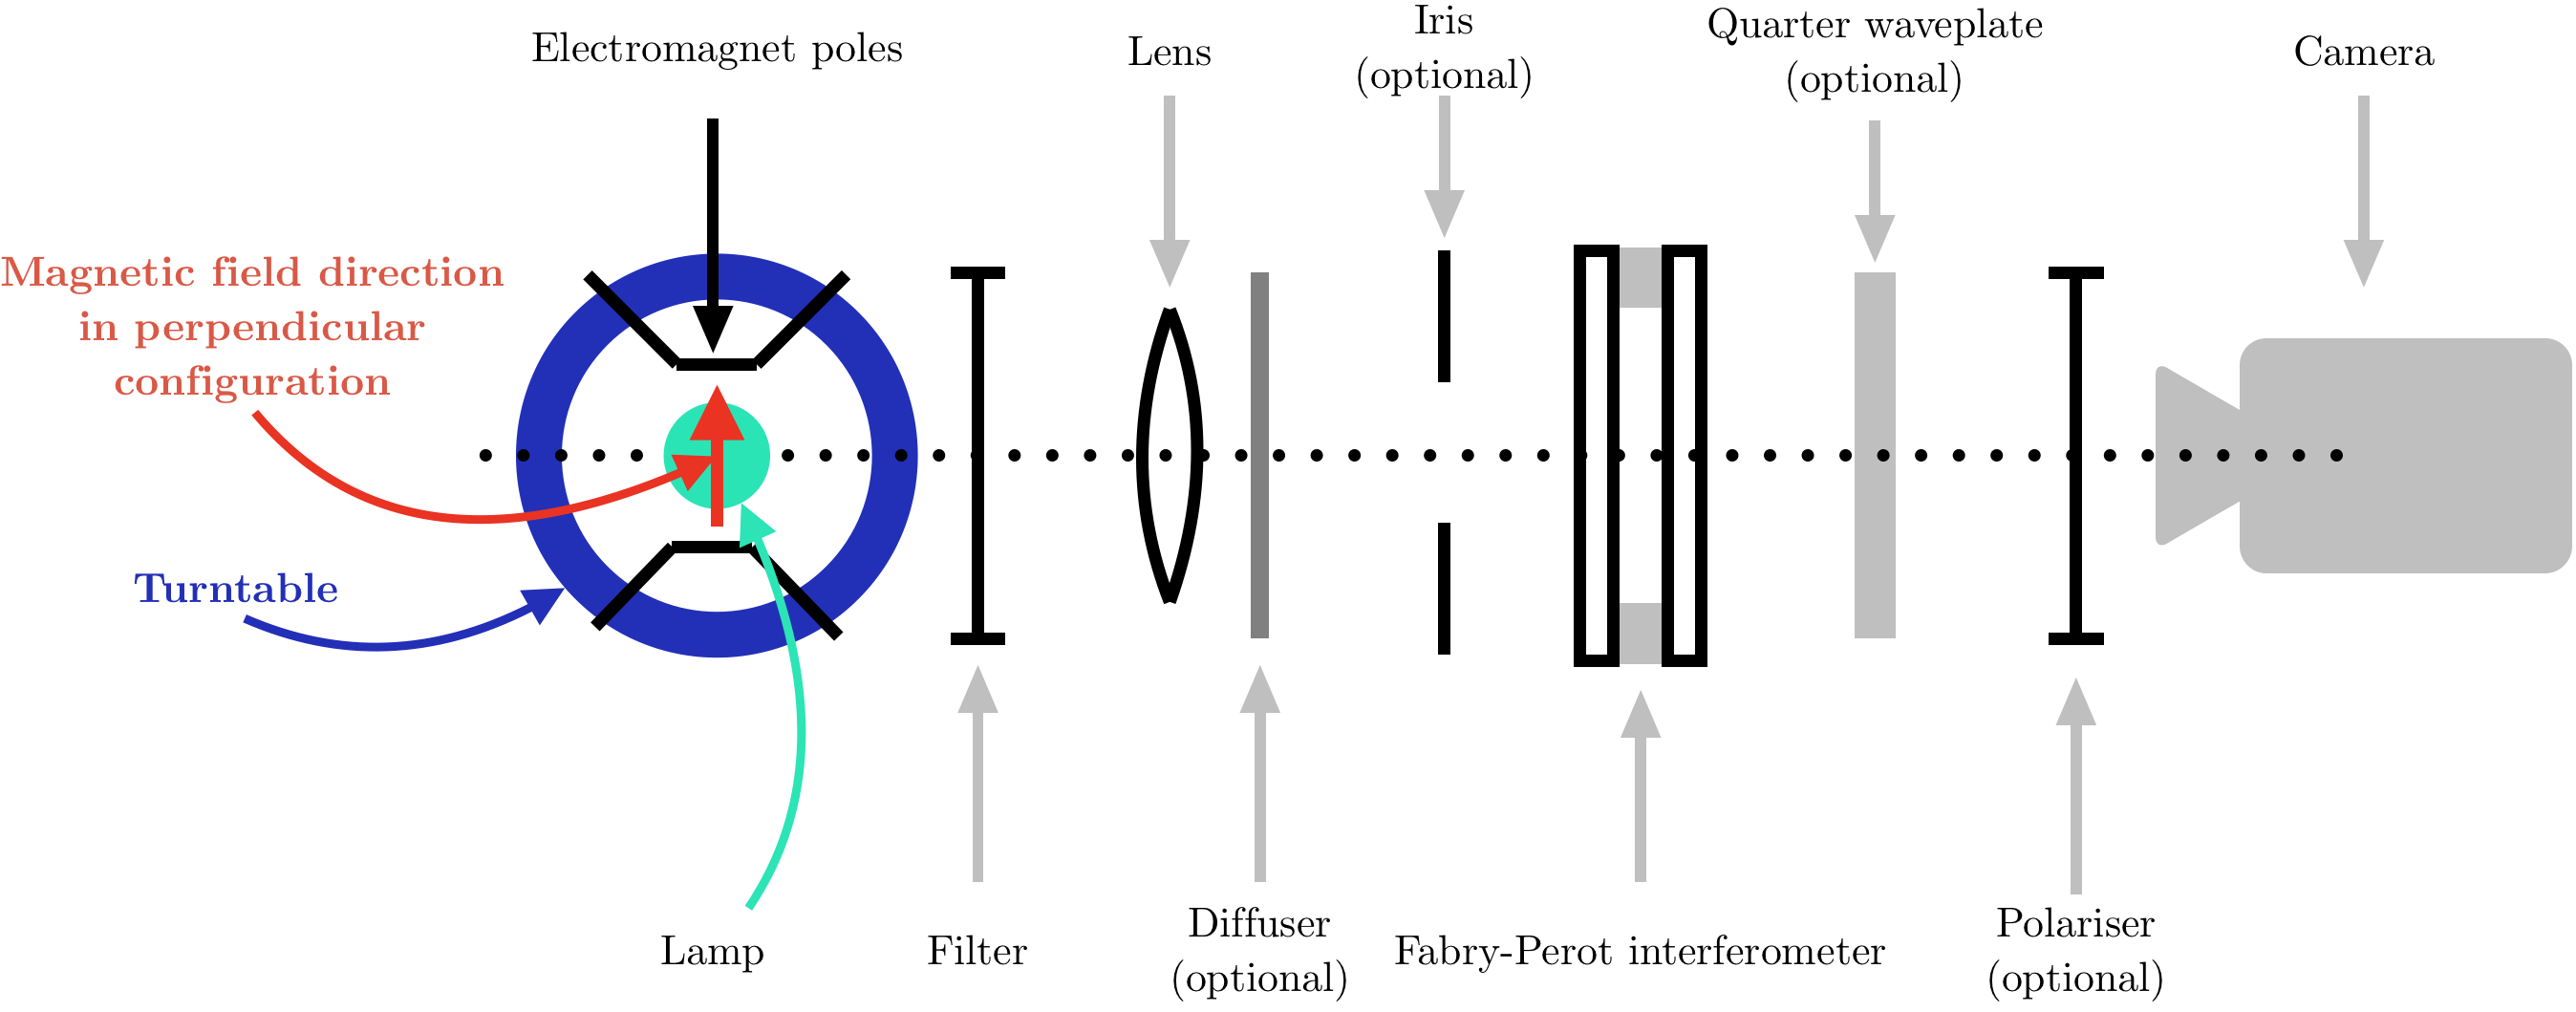
\includegraphics[width=0.8\linewidth]{setup2.png}
    \captionsetup{justification=centering}
    \caption{Diagram of the experimental setup. See Appendix \ref{sec: app setup}, Fig. \ref{fig: setup photo} for an image of the setup}
    \label{fig: setup}    
\end{figure}

\subsection{B-field and polariser calibration}
The current in the electromagnets was correlated with the magnetic field obtained. We used a Hall effect sensor to measure the magnetic field in which the lamp will be placed. We used several readings at different currents to obtain the relation between the current in the coils and the field obtained (Fig. \ref{fig:IvsB}). For each current value we were able to measure a range of magnetic field values, because the field in between the two cores was not perfectly uniform. We tried to measure the value at the centre point and we estimated the error on the measurement based on how much the field changed as we moved the Hall effect probe in between the two iron cores. The fact that the field was not linear contributed to the widening of the observed lines. It was also observed that there was a residual magnetic field, because of the iron cores. This was accounted for when fitting the measurements. We were able to obtain a stronger field with the hollow iron cores (Fig. \ref{fig:IvsB hollow}) because the cores were mounted around $30\%$ closer together.

The scale on the polariser (ranging from 0 to 360 degrees) was correlated with the direction of E-field using Brewster's angle. Vertical polarisation corresponds to 135 degrees (and horizontal at a $45^\circ$ angle). We used the calibrated polariser to identify the polarisation of the lines under perpendicular observation. We identified the $\sigma$ component as the one with polarisation perpendicular to the B field and the $\pi$ component as polarised longitudinally. The order (and position) of the split $\sigma$ and $\pi$ components is as predicted by the Zeeman effect. Under longitudinal observation we were not able to observe $\pi$ components (as predicted), and we were able to find that the $\sigma$ components have circular polarisation. The handedness of the circular polarisation was determined in section \ref{sec: e/m ratio} by using a $543 \si{nm}$ quarter-wave plate. 

\subsection{Fabry-Perot interferometer}
A Fabry-Perot interferometer consists of two parallel and highly reflective transparent plates, typically glass, separated by a small distance. When light passes through these plates, it creates interference patterns, resulting in concentric circular fringes. These fringes indicate interference between multiple light paths, with higher fringe orders towards the center. The free spectral range of the interferometer refers to the spacing between adjacent fringes, determining the range of wavelengths it can resolve (see equation \eqref{eq: instr resolution}. 
Finesse, on the other hand, represents the sharpness of the fringes, indicating how well-defined they are. Finesse is related to the reflectivity of the mirrors by \eqref{eq: finesse}. 

The plates of the Fabry-Perot can be adjusted with two piezoelectric crystals (on the two axes). We could find the position where the plates of the interferometer are parallel by moving the observer in the left-right and up-down directions and checking if the interference pattern changes. We started with the lens such that the light bulb is in focus, but later in the experiment we also tried moving it to obtain a more diffuse image of the bulb. This helped with the visibility of the interference ring. The camera focus was set to $\infty$ and the aperture was open all the way to maximise the light hitting the sensor. 
\label{sec: d}

The optical path $nd = 4.42 \pm 0.17 \si{mm}$ between the plates of the Fabry-Perot was measured using the pattern observed for the red line ($\lambda = 644$ nm) and using the formula \eqref{eq: d}, where $r_m$ is the radius of the $m^{\text{th}}$ order and $f_c$ is the focal distance of the camera. We assumed that the refractive index does not significantly change as function of wavelength over the range tested. The interferometer needed to be re-calibrated after every set of measurements in order to keep the resolution as high as possible. This was probably caused by thermal expansion caused by the heating of the piezoelectric components. 
\begin{equation}
    nd = \lambda \frac{f_c^2}{r_m^2-r_{m-1}^2} \label{eq: d}
\end{equation}

Despite changing the position of the plates when re-calibrating the interferometer in order to maintain the sharp image, we were not able to measure a change in the distance between the plates. This is because our error on distance $d$ is on the order of $0.17 \si{mm}$ and the adjustments made during re-calibration are much smaller than the error margin, on the order of the wavelength $\lambda \approx 500 \si{nm}$. We conclude therefore that one should not be concerned with remeasuring the distance between the plates. It can also be safely assumed that the refractive index for air stays constant ($n=1$), as its dependence on temperature and wavelength is much smaller that other sources of error in the experiment \cite{Polyanskiy2024}. 

\subsection{Instrumental resolution}
To put into perspective the order of magnitude of the line splitting values measured, we can take an average magnetic field of $B = 0.3$T and a g-factor of $g_{eff}=1$, which give a splitting of $\Delta \nu = 14 \mathrm{m}^{-1}$. 
 
There are four main factors that limit the maximum wavenumber measurement resolution that can be obtained: Doppler broadening \ref{item: doppler}, Airy distribution \ref{item: resolution}, the non-uniformity of the B-field \ref{item: field} and the mirror flatness \ref{item: flattness}. 
\begin{enumerate}[label=(\alph*), ref=(\alph*)]
  \item \label{item: doppler} The spectral width of a line will be dominated by Doppler broadening. By assuming a Boltzmann distribution $f(v) = \sqrt{\frac{m}{2 \pi k T}} e^{-\frac{mv^2}{2kT}}$ for the particles, and by substituting the velocity $v$ from the Doppler shift equation $f = f_0 (1+v/c)$, we were able to recognise a Gaussian distribution with the FWHM of: 
  \begin{equation}
      \delta \nu_{\mathrm{Dopp}} = \sqrt{\frac{8 k T \ln{2}}{mc^2}} \nu_0
  \end{equation}
  where $m$ is the mass of an atom, $T$ is the temperature and $\nu_0$ is the wavenumber of the peak of the distribution. By introducing the temperature of $T = 500 \si{K}$ into the equation, which is in line with the literature \cite{doi:10.1098/rspa.1936.0108}, we obtained an expected broadening in the range of:
  \begin{equation}
      \delta \nu_{\text{Dopp Cd red}} = 2.4 \si{m^{-1}} \label{eq: nu doppler}
  \end{equation}
  \begin{equation}
      \delta \nu_{\text{Dopp Hg blue}} = 3.5 \si{m^{-1}}
  \end{equation}
  \item \label{item: resolution} In theory, the resolution of a Fabry-Perot interferometer is related to the finesse $F$ of the instrument by: 
  \begin{equation} \label{eq: instr resolution}
      \delta \nu_{\text{instr}} = \Delta \nu_{\text{FSR}} F^{-1} = \frac{1}{2d} F^{-1}
  \end{equation}
  where $\Delta \nu_{\text{FSR}}$ is the free spectral range of the instrument. According to \cite{FabryPerotEtalonGuide} we are expecting the reflectance of the mirrors of the Fabry-Perot to be $R = 0.95$. This is close enough to $1$ to approximate the finesse to be given by equation \eqref{eq: finesse}. 
  \begin{equation}
      F = \frac{\pi R^{\frac{1}{2}}}{1 - R} \label{eq: finesse}
  \end{equation}
  This results in a theoretical maximum instrumental resolution limit of: 
  \begin{equation}
      \delta \nu_{\text{instr}} = 1.6 \si{m^{-1}}
  \end{equation}
  \item \label{item: field} The magnetic field in the space between the iron cores was not perfectly uniform: edge effects make the field lines diverge and the field weaker at the centre of the gap between the cores. We were able to measure the variation of the magnetic field with the Gauss meter (Fig. \ref{fig:IvsB}) and it is of the order of $5 \si{mT}$ for the highest magnetic fields achievable with this setup. We estimated the broadening resulting from the Zeeman effect caused by a spectrum of B-fields using equation \eqref{eq: splitting} to be at most: 
  \begin{equation}
      \delta \nu_{\text{B}} = 0.5 \si{m^{-1}}
  \end{equation}
  This value corresponds to a $g_{eff} = \pm 2$ value, and because it is much smaller than the other sources of line broadening, it will not significantly contribute to the final total resolution limit of the instrument. 
  \item \label{item: flattness} The flatness of the mirrors is essential in obtaining a sharp image, as a deviation of just $\lambda / 2 \approx 250 \si{nm}$ creates destructive interference. This is why we re-calibrated the mirror alignment after every set of measurements. Since we used a mirror surface with a dimension on the order of $1 \si{cm}$, any curvature with a radius lower than $R \approx 400 \si{m}$ will make measurements impossible. We were not able to estimate the flatness of the mirror, but results (section \ref{sec: resolution measurement}) indicated this plays an important role in determining the total instrumental resolution limit (equation \eqref{eq: nu tot prediction}). 
\end{enumerate}
The resulting total resolution limit of the instrument was estimated by adding in quadrature the individual errors, and is predicted to be at most: 
\begin{equation} \label{eq: nu tot prediction}
    \delta \nu_{\text{total}} = \sqrt{\delta \nu_{\text{Dopp}}^2 + \delta \nu_{\text{instr}}^2 + \delta \nu_{\text{B}}^2} = 3.9 \si{m^{-1}}
\end{equation}

\subsection{Measurement} \label{sec: measuremet}
The fundamental equation that predicts the angular position of the maxima in a Fabry-Perot interferometer is:
\begin{equation}
    m = 2 \nu n d \cos{\theta} 
    \approx 2 \nu n d (1 - \theta^2/2)
    \approx 2 \nu n d (1 - \frac{r^2_m}{2f^2_c})
    \label{eq: order}
\end{equation}
where $m$ is the interference order and $\theta  \approx r_m/f_c$ is the angle. By subtracting equations \eqref{eq: order} for orders $m$ and $m + 1$ we find that: 
\begin{equation}
    r^2_m - r^2_{m+1} = f^2_c/\nu n d
\end{equation}
For a different component at position  $\nu + \Delta \nu$, where $\Delta \nu$ is the line splitting, equation \eqref{eq: order} becomes: 
\begin{equation}
    m = 2 (\nu + \Delta \nu) n d (1 - \frac{r'^2_m}{2f^2_c})
\end{equation}
Combining these equations we find the splitting $\Delta \nu$ to be: 
\begin{equation}
    \Delta \nu = - \frac{1}{2nd} \frac{r^2_m - r'^2_m}{r^2_m - r'^2_{m+1}}
    \label{eq: nu measurement}
\end{equation}
where $r_m$ is the radius of the inner component, $r'_m$ is the radius of the outer component for the order $m$, and $nd$ is the optical path \eqref{eq: d}. The radii of the rings in the interference pattern are measured using the Thor Labs software (Fig. \ref{fig: d measurement}). The software is used to control shutter and gain of the camera to obtain the desired image brightness. We used the circular measure tool to manually fit circles to the maxima in the interference pattern and the software provides the radius of the circles in number of pixels. 

%-------------------------------------------------------------------


\section{Error analysis} \label{sec: err}
The leading source of error on the splitting measurements was the $3.8\%$ error on the measurement of the distance $d$ between the plates. Another significant source of error was random error from the interference maxima radius measurement. We calculated this as standard deviation of the individual measurements. There was also a $1\%$ error on the correlation between field strength and current. As we only directly measured current, this error affected all splitting measurements. These errors were be considered independent and the final result is linearly dependent on these parameters, therefore we combine the percentage errors by adding them in quadrature.

Numerical errors were considered, but they turn out to be insignificant: In equation \eqref{eq: order} it was assumed that $\theta$ is small \eqref{eq: small theta}, and $\theta^3$ order and higher terms were neglected ($\theta^3 \approx 10^{-4}$). 
\begin{equation}
    \theta \approx \frac{\mathrm{\#\ of\ pixels} \times \mathrm{pixel\ width}}{\mathrm{focal\ distance}} \approx \frac{700 \times 5.86 \si{\mu m}}{75 \si{mm}}
    \approx 0.05 \ll 1
    \label{eq: small theta}
\end{equation}

%-------------------------------------------------------------------

\section{Results} \label{sec: results}

\subsection{Cadmium red transition - normal Zeeman effect} \label{sec: Cd red}
We first studied the $5^1 D_2\rightarrow 5^1 P_1$ transition for the cadmium red line. We used Table \ref{tab: quantum_numbers} and equation \eqref{eq: g eff} to find the possible values for the effective g-factor to be $g_{eff} = -1, 0, 1$. This means that we expected the line to split into 3 components, with the splitting given by equation \eqref{eq: splitting}. The theoretical value of the linear line splitting $\Delta \nu $ as function of magnetic field $B$ for $g_{eff} = \pm 1$ is: 
\begin{equation}
    \text{Theoretical value: } \frac{\Delta \nu}{B} = 46.7 \, \si{m^{-1}.T^{-1}}
\end{equation}
We were able to observe that, as the magnetic field strength is increased, the maxima split into 3 components: the $\pi$ component ($g_{eff} = 0$) remained in place and the two $\sigma$ ($g_{eff} = \pm 1$) components moved apart on each side of the $\pi$ line. The splitting was predicted to be symmetric between the ($g_{eff} = \pm 1$) pair, this was also experimentally confirmed. The magnitude of the splitting was plotted in Figure \ref{fig: Cd red}, with the linear dependence measured using a linear fit with $0$ intercept (equation \eqref{res: Cd red}). 
\begin{equation}
    \text{Measured value: } \frac{\Delta \nu}{B} = 46.5 \pm 3.6 \, \si{m^{-1}.T^{-1}}
    \label{res: Cd red}
\end{equation}
\begin{figure}
    \centering
    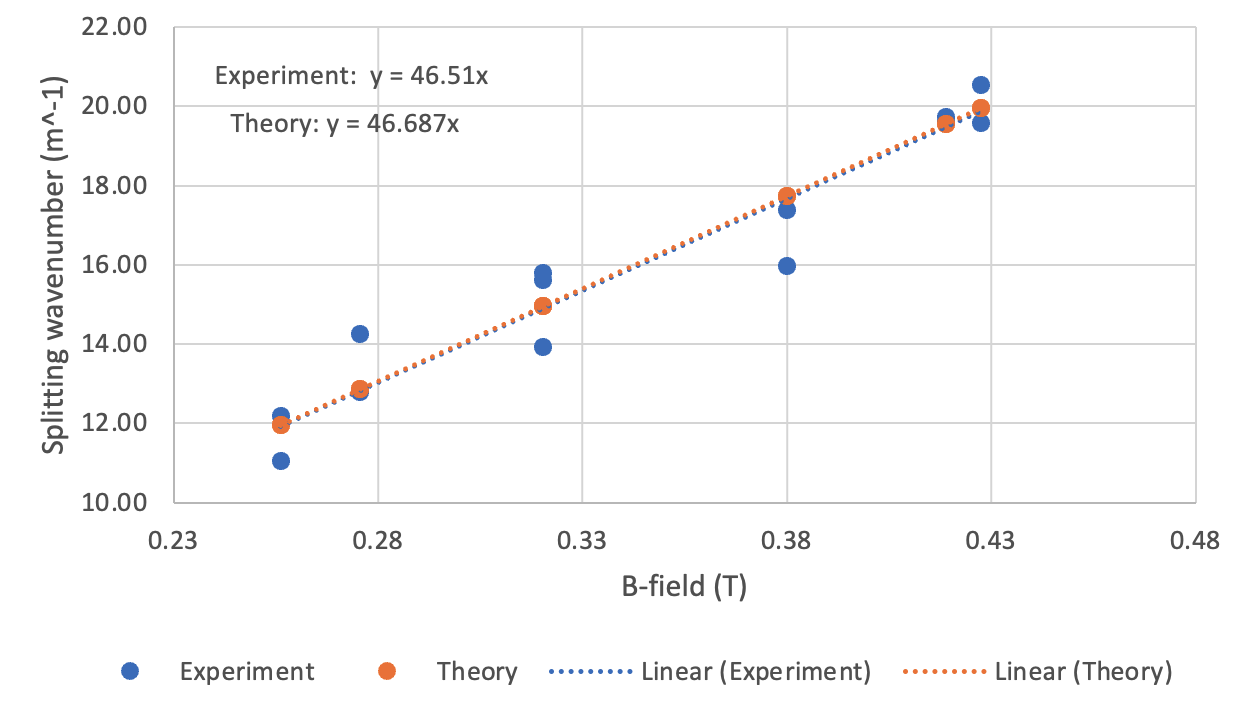
\includegraphics[width=0.6\linewidth]{Cd red.png}
    \caption{Line splitting for the $\sigma$ polarised line due to the Zeeman effect in the cadmium red transition, $5^1 D_2\rightarrow 5^1 P_1$, $\lambda = 643.85\si{nm}$}
    \label{fig: Cd red}
\end{figure}


\subsection{Electron charge to mass ratio} \label{sec: e/m ratio}
An interesting use of the experiment performed in section \ref{sec: Cd red} is that we can employ the result \eqref{res: Cd red} to derive the charge to mass ratio of the electron. The formula for the Bohr magneton $\mu_B = e \hbar / (2 m_e)$ is introduced into equation \eqref{eq: splitting}, and after using that $g_{eff} = 1$ for this transition, we obtain: 
\begin{equation}
    \frac{e}{m_e} = 4 \pi c \frac{\Delta \nu}{B} = (-1.75 \pm 0.14) \times 10^{11} \si{C.kg^{-1}}
\end{equation}
This is in agreement with the theoretical value \cite{CODATA2018}: 
\begin{equation}
    \frac{e}{m_e} = -1.75882001076(53) \times 10^{11} \si{C.kg^{-1}}
\end{equation}
Interestingly, it is also possible to determine the sign of the electron charge. We used a beetle as reference for left hand polarised light. The beetle reflects bright green left-hand polarised light. Therefore we determined that the outer ring in the interference pattern were LH polarised and the inner ones were RH polarised. These measurements were done with a longitudinal setup, parallel to the magnetic field. We used a compass to determine that the B-field vector was in the direction of the photon momentum. Outer ring is higher energy ($\Delta \nu > 0$), and $ \Delta m_J = 1$ corresponds to RH polarisation. By substitution into equation \eqref{eq: splitting}, this result confirms that electrons have negative charge. 

\begin{figure}[h!]
    \centering
    \begin{subfigure}{0.47\linewidth}
        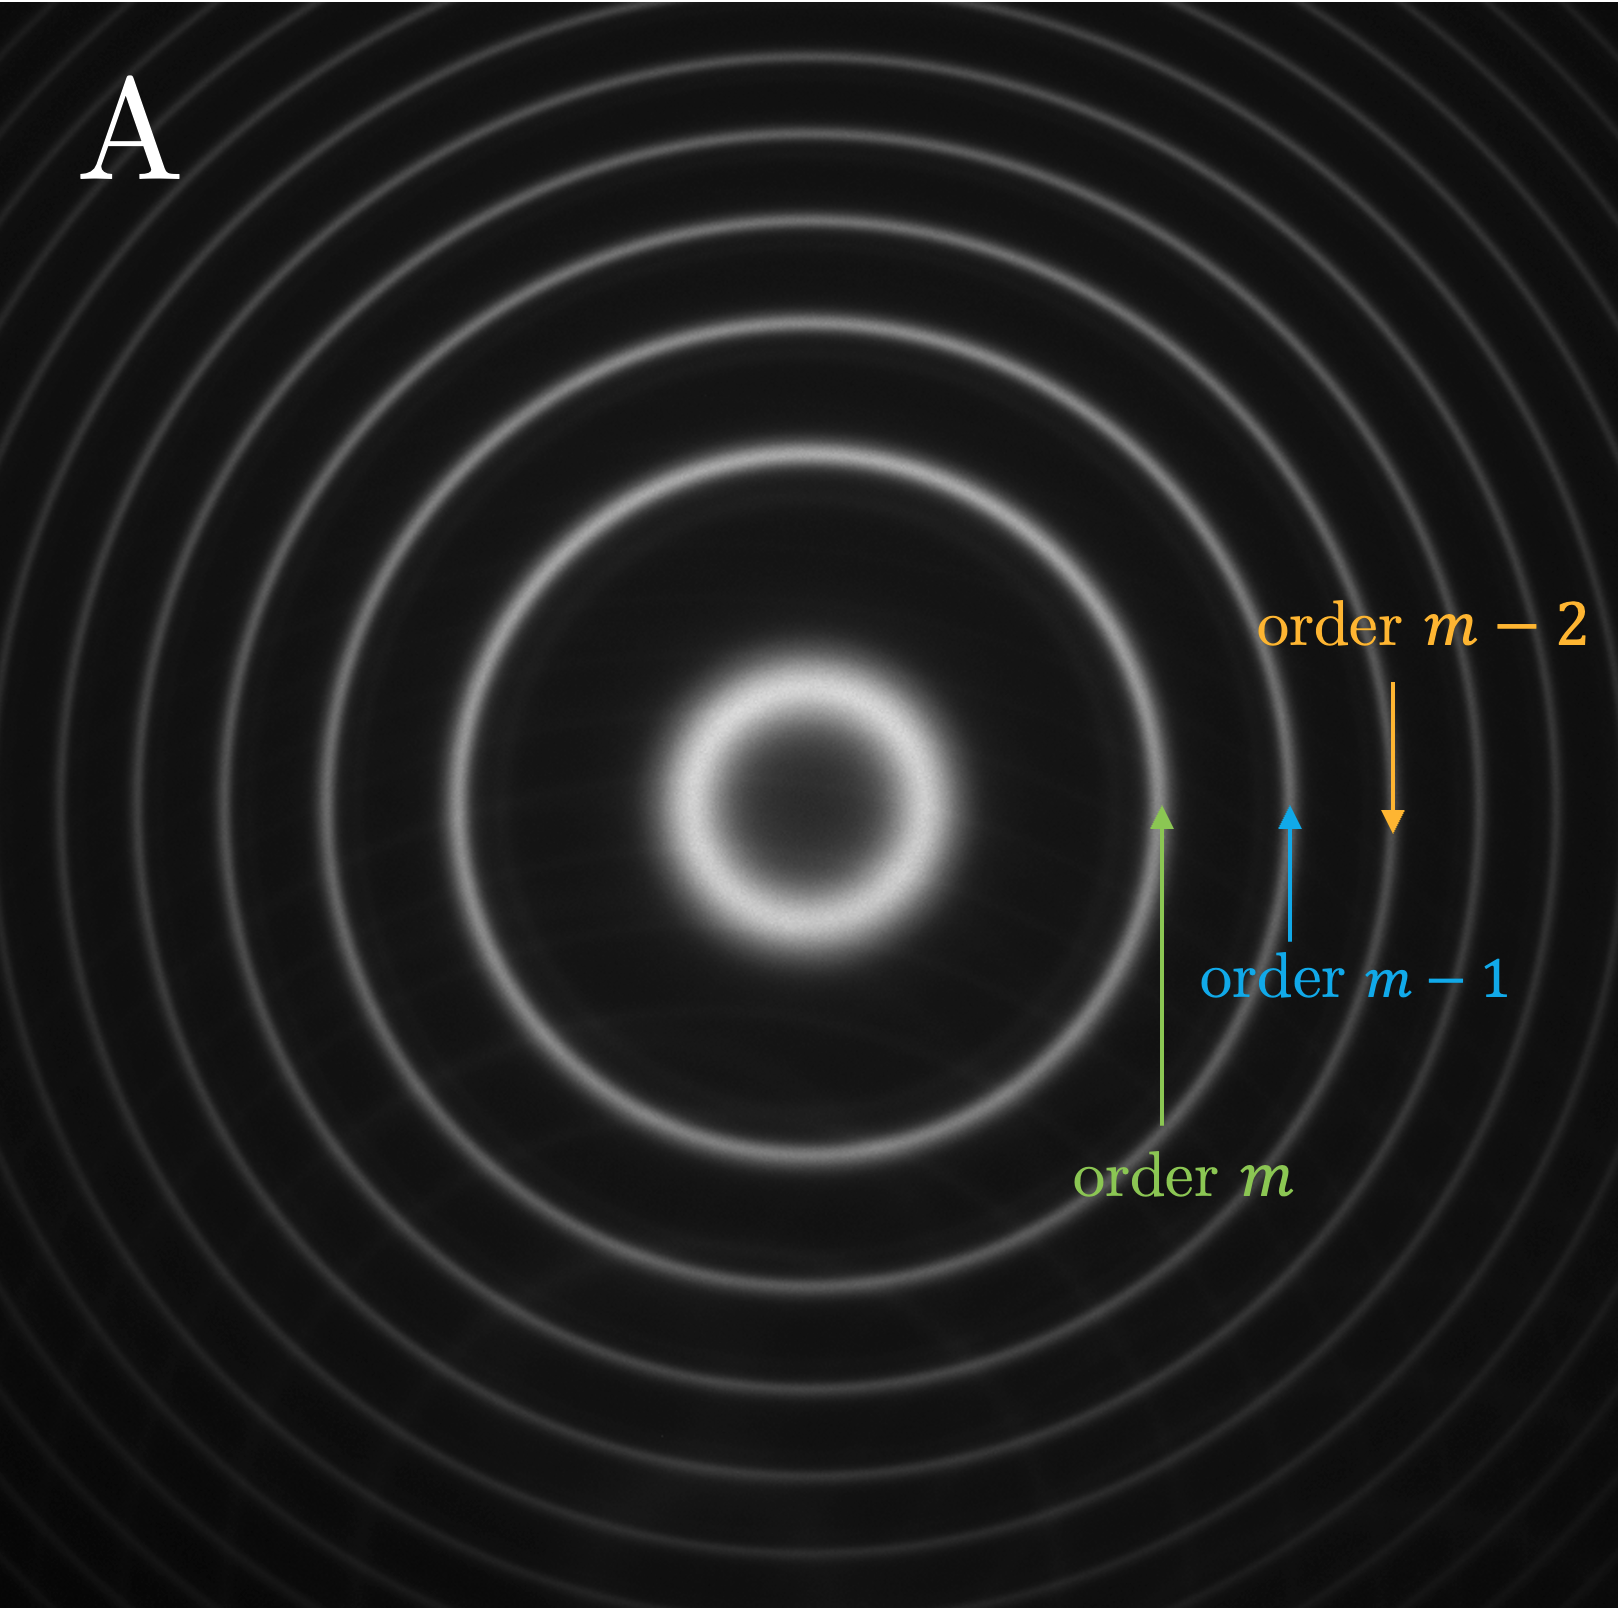
\includegraphics[width=\linewidth]{Cd green/A2.png}
    \end{subfigure}
    \begin{subfigure}{0.47\linewidth}
        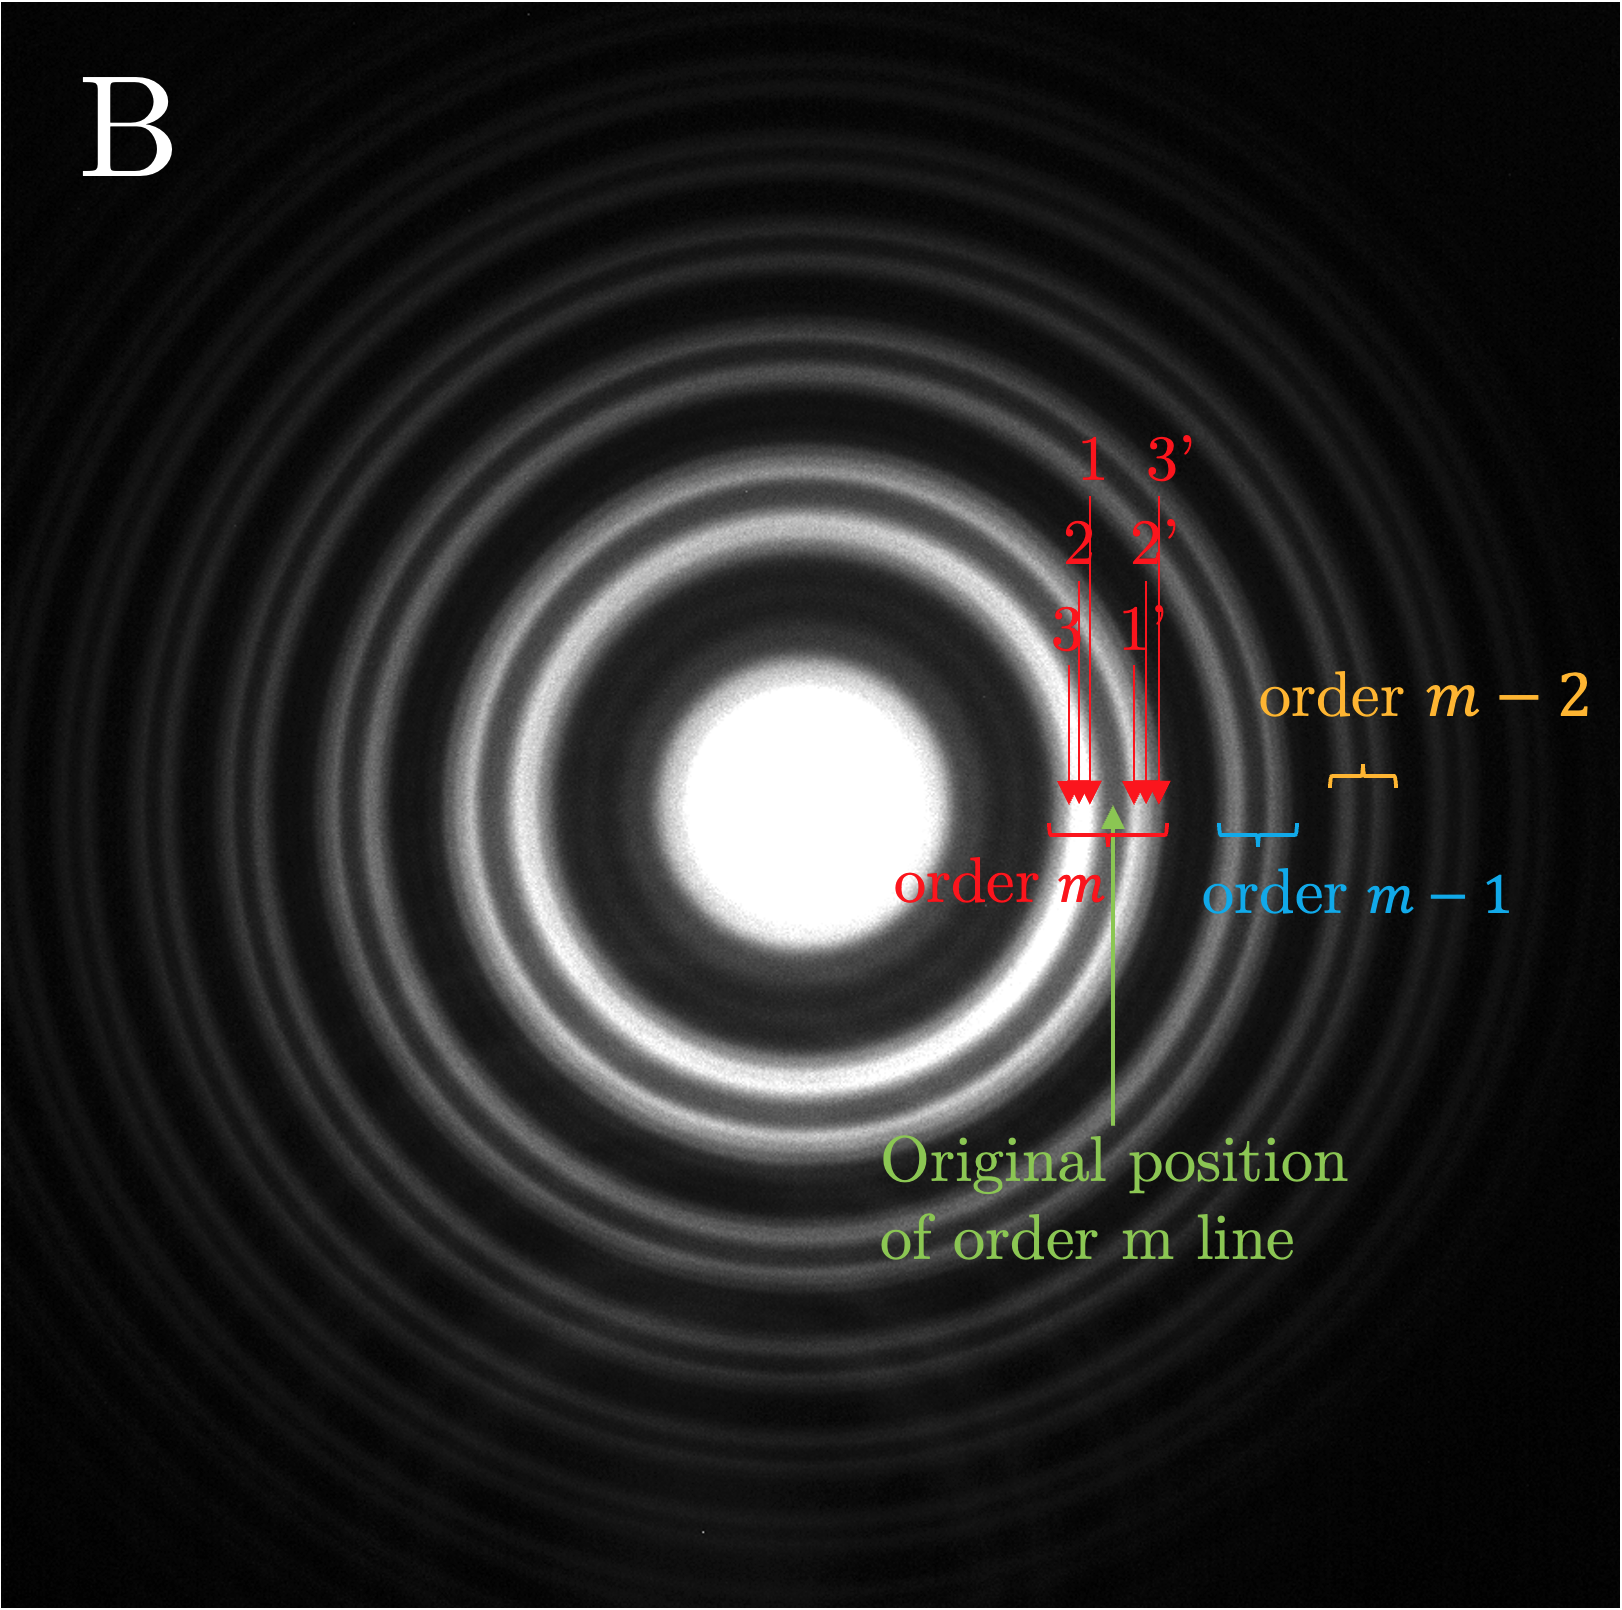
\includegraphics[width=\linewidth]{Cd green/B2.png}
    \end{subfigure}
    \begin{subfigure}{0.47\linewidth}
        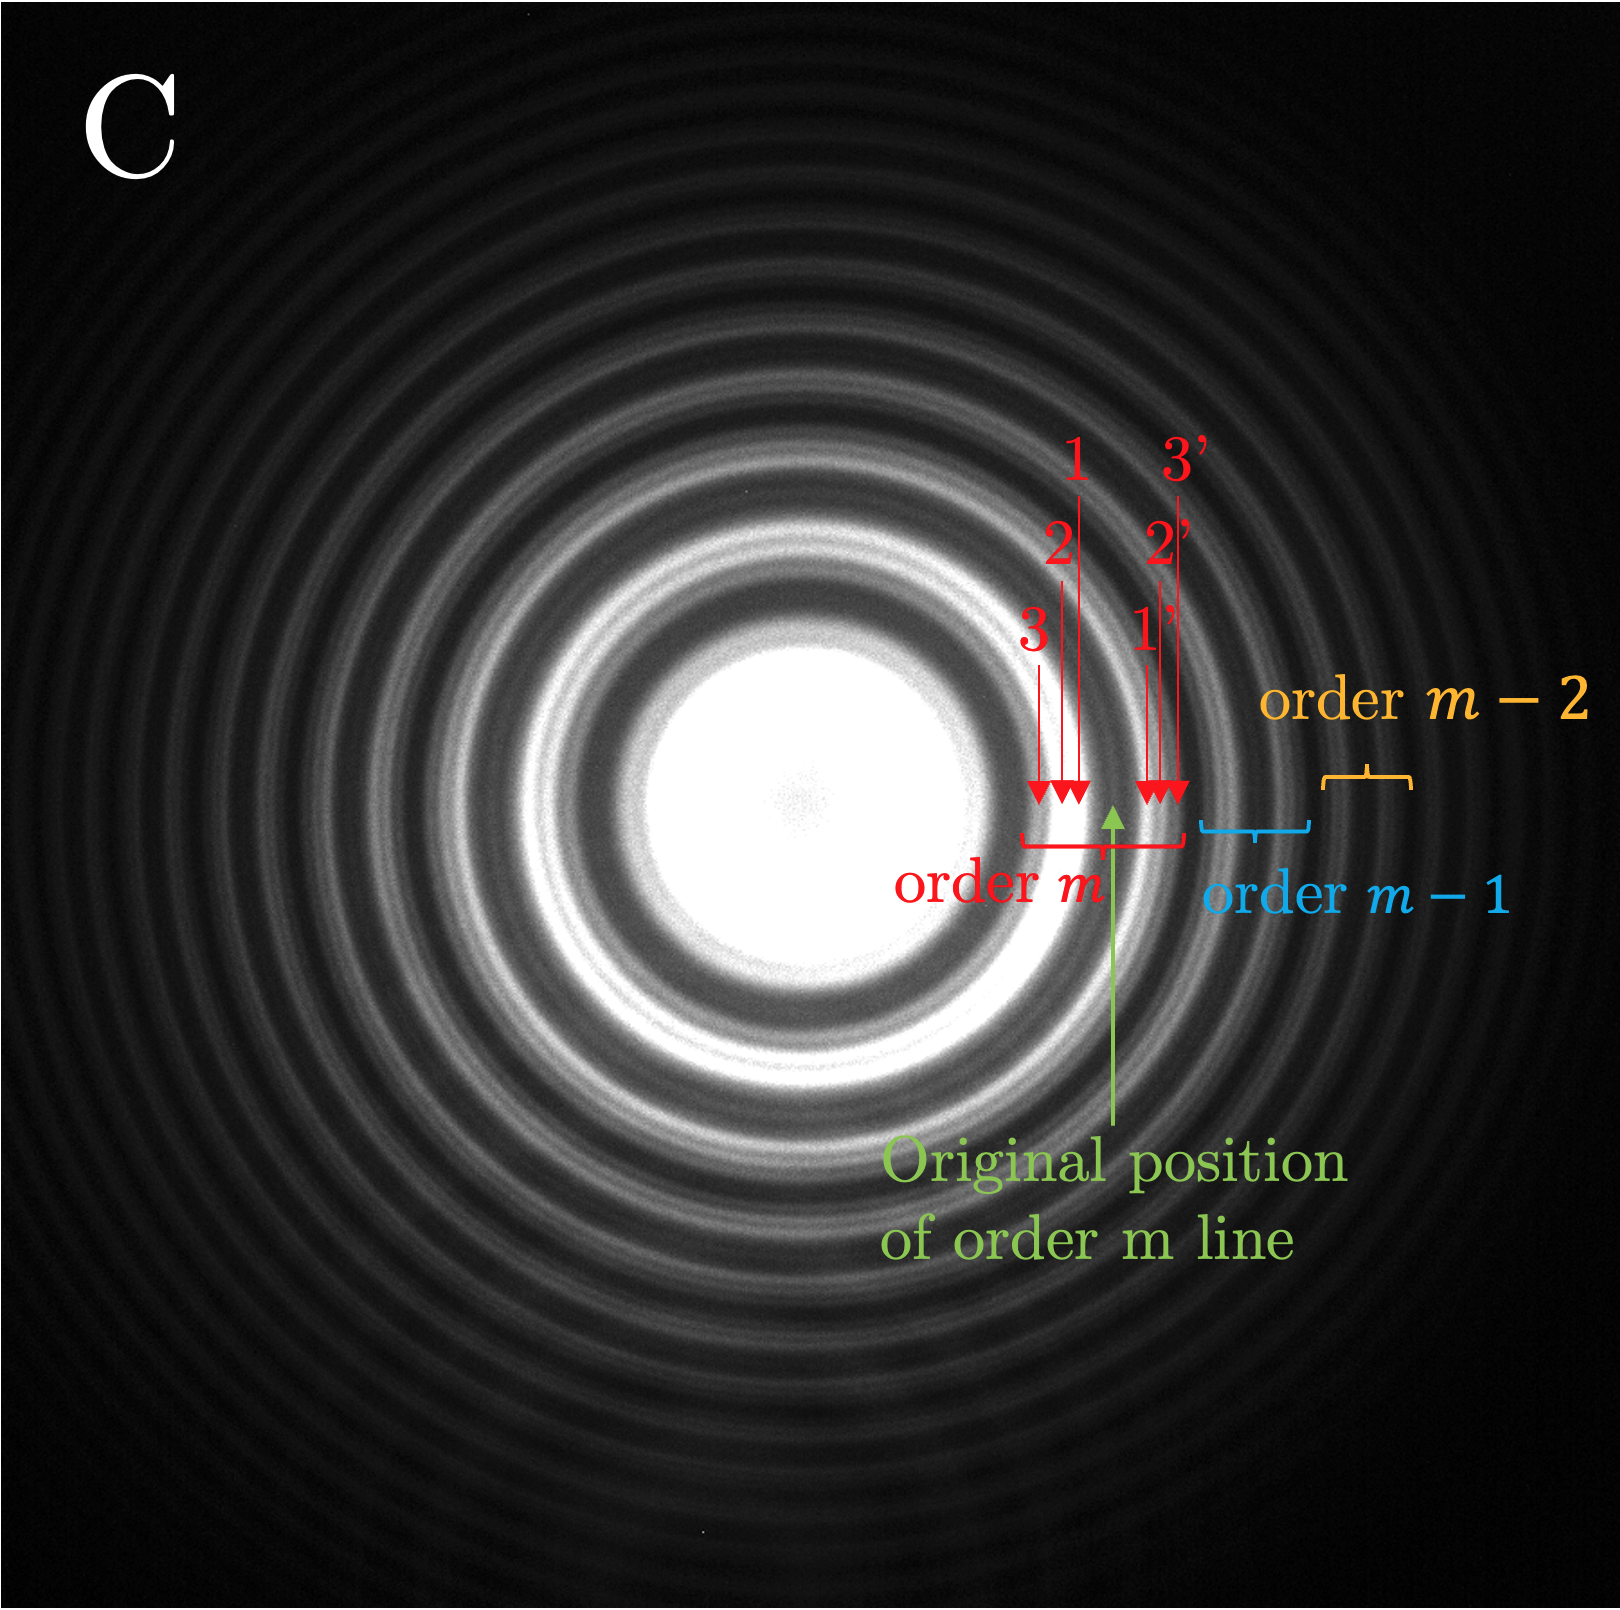
\includegraphics[width=\linewidth]{Cd green/C2.png}
    \end{subfigure}
    \begin{subfigure}{0.47\linewidth}
        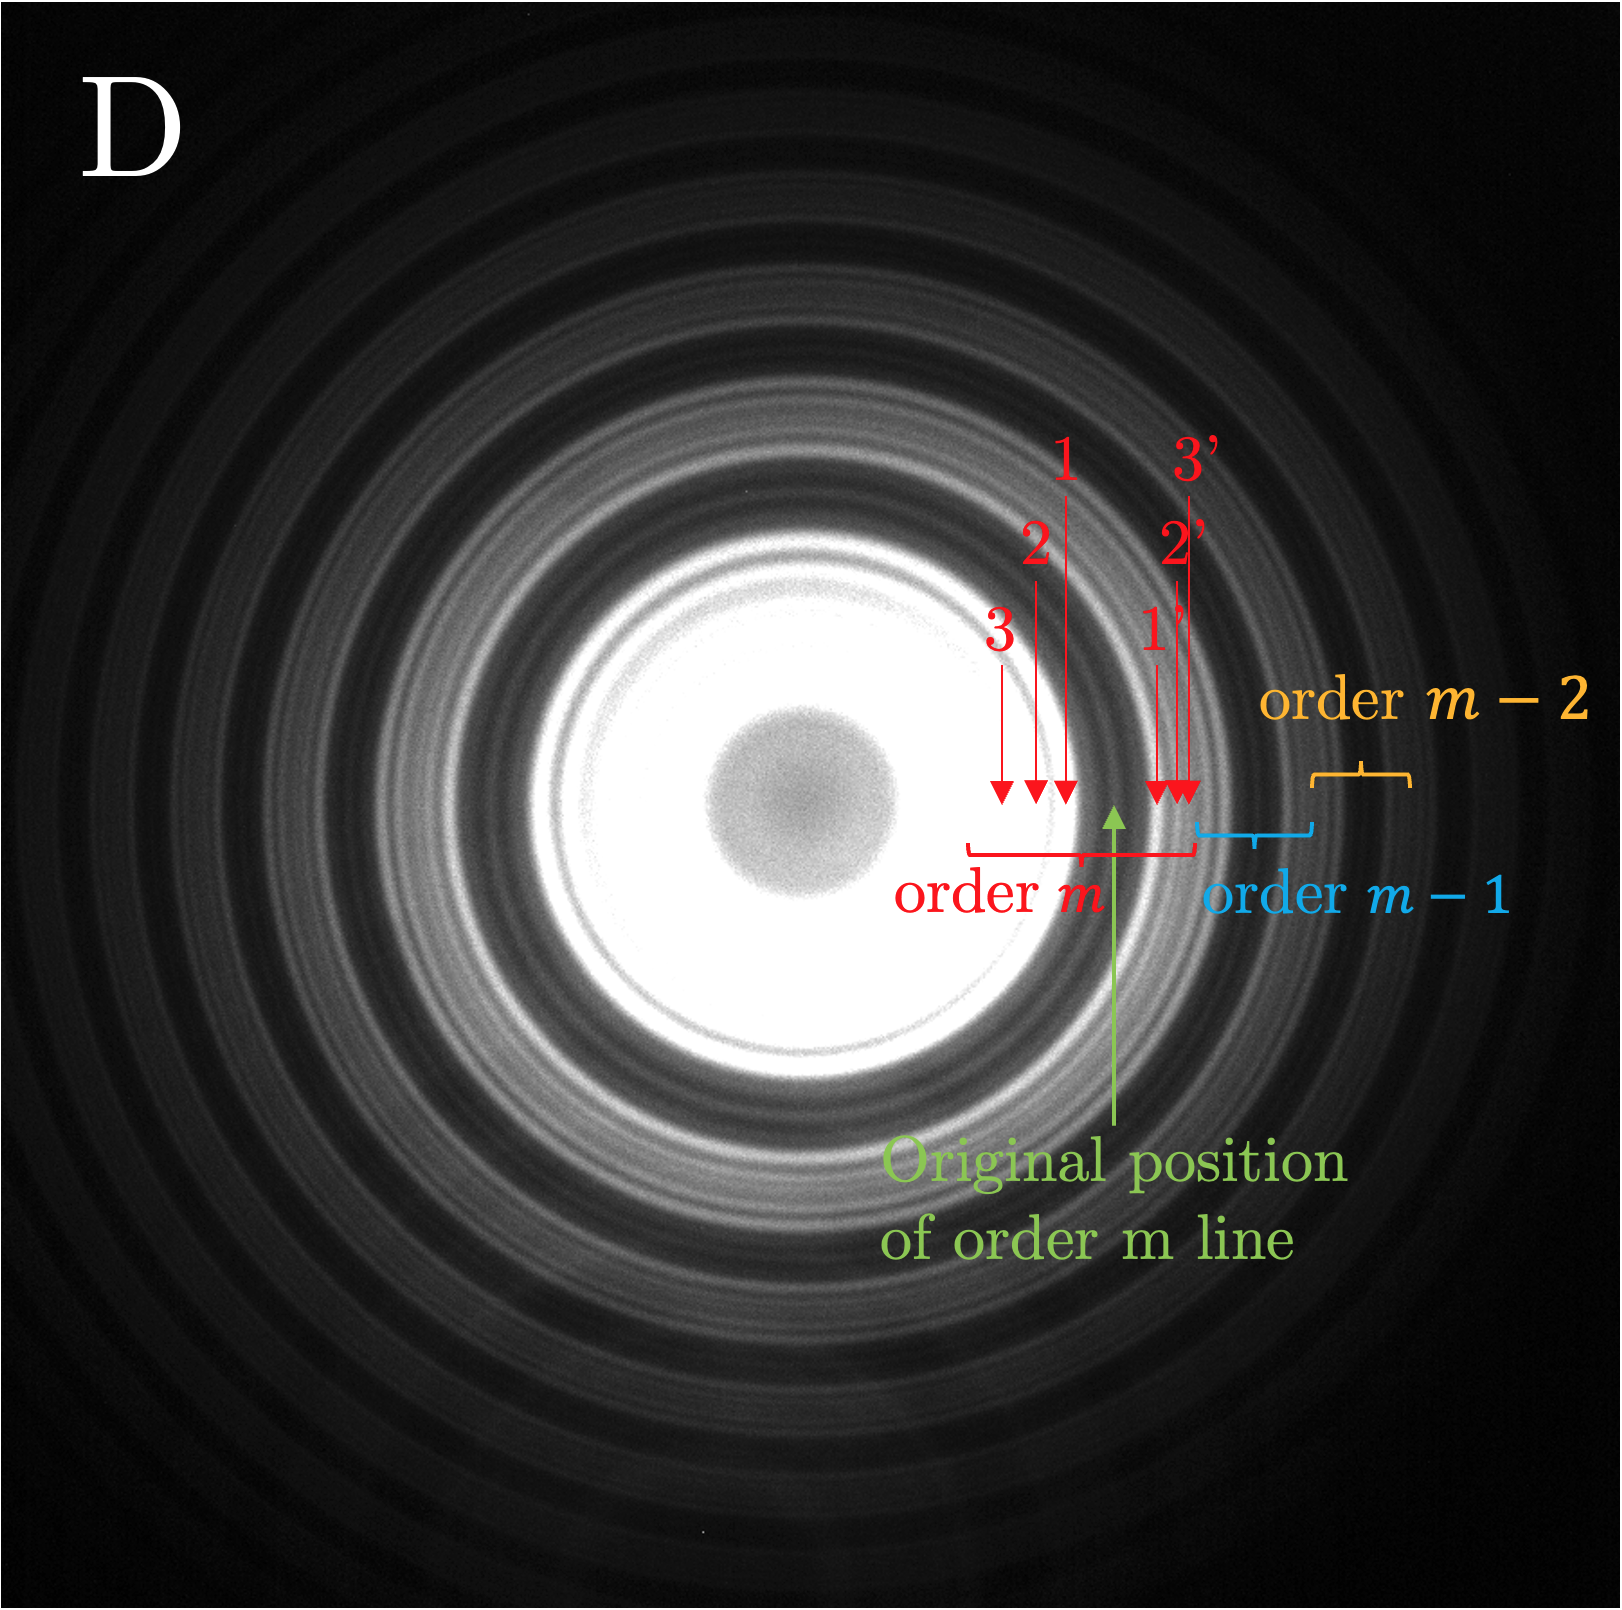
\includegraphics[width=\linewidth]{Cd green/D2.png}
    \end{subfigure}
        \captionsetup{justification=centering}
    \caption{Fabry-Perot interferometer images of the cadmium green line observed along the field lines (parallel observation). Only the 6 $\sigma$ polarised lines are visible under longitudinal observation. Magnetic field is increased from $0.03 \si{T}$ in Fig. A, to $0.46 \si{T}$ in Fig. B, to $0.54 \si{T}$ in Fig. C, and up to $0.62 \si{T}$ in Fig. D. The lines are not resolved for field lower that in Fig B, and the different orders start overlapping for fields higher than in Fig D. The labels 3, 2, 1, 1', 2', 3' correspond to the $g_{eff} = -2, -1.5, -1, 1, 1.5, 2$ values respectively (see Table \ref{tab: Cd green g_eff}). The rings labelled with the primed number are referred to as outer rings and the non-primed are inner rings.}
    \label{img: Cd_green_sigma_increasing_field}
\end{figure}
\subsection{Cadmium green transition - anomalous Zeeman effect} \label{sec: Cd green}
The $5^3 S_1\rightarrow 5^3 P_2$ transition, for the cadmium green line, exhibits the anomalous Zeeman effect: the spin of the electrons couple together and the interaction involves both the orbit and angular momentum and the spin angular momentum. The anomalous Zeeman effect splits the spectral line in more than three components that are not necessarily equally spaced apart. The effective g-factor values, derived using Table \ref{tab: quantum_numbers} and equation \eqref{eq: g eff} are shown in Table \ref{tab: Cd green g_eff} together with their polarisation. Having 9 different possible values for $g_{eff}$ means that we expect the line to split into 9 components, with the splitting given by equation \eqref{eq: splitting}.

\begin{table}[h!]
    \centering
    \begin{tabular}{c|ccccc}
    \toprule
        Observation & Polarisation  & \( g_{eff} \) & No. of independent & Measured splitting  & Theoretical splitting \\
        configuration & & & measurements & $\Delta \nu / B$ ($\si{m^{-1}.T^{-1}}$) & $\Delta \nu / B$ ($\si{m^{-1}.T^{-1}}$) \\
    \midrule
        perpendicular & \( \pi \) & 0 & - & no splitting & 0\\
        perpendicular & \( \pi \) & $\pm 0.5$ & 12 & $22.4 \pm 1.0$ & 23.4\\
        perpendicular & \( \sigma \) & $\pm 1$ & 8 & $44.7 \pm 2.1$ & 46.7\\
        perpendicular & \( \sigma \) & $\pm 1.5$ & 8 & $63.8 \pm 2.9$ & 70\\
        perpendicular & \( \sigma \) & $\pm 2$ & 8 & $85.1 \pm 3.9$ & 93.4\\
        parallel & \( \sigma \) & $\pm 1$ & 9 & $43.4 \pm 2.0$ & 46.7\\
        parallel & \( \sigma \) & $\pm 1.5$ & 9 & $69.2 \pm 3.3$ & 70\\
        parallel & \( \sigma \) & $\pm 2$ & 7 & $89.8 \pm 4.1$ & 93.4\\
    \bottomrule
  \end{tabular}
    \captionsetup{justification=centering}
  \caption{Cadmium green line: measured line splitting wavenumber $\Delta \nu$ dependence on magnetic field $B$ and $g_{eff}$ factor in the $5^3 S_1\rightarrow 5^3 P_2$ transition. The calculated values of \(g_{eff}\) are shown with the corresponding polarisation according to the Zeeman effect predictions}
  \label{tab: Cd green g_eff}
\end{table}
This is indeed what we observed: when the magnetic field is applied, the line splits into 9 components. A polariser (or longitudinal observation) is used to select only the $\pi$ or $\sigma$ polarisations in order to more easily perform the measurements (see Fig. \ref{img: Cd_green_sigma_increasing_field} with only $\sigma$ polarisations). Our experiment verifies that the measured line splitting is the same in both longitudinal and perpendicular configurations. 

\subsection{Mercury green transition} \label{sec: Hg green}
The splitting of the mercury green line (Fig. \ref{fig: Hg green sigma}, \ref{fig: Hg green pi} and Table \ref{tab: Hg green results}, transition $7^3 S_1 \rightarrow 6^3P_2$) is the same as in the cadmium green (transition $5^3 S_1 \rightarrow 5^3P_2$), within error, and in agreement with the theory. This confirms that the line splitting has no measurable dependence on the principal quantum number $n$ or on other atomic properties of the material such as electron number $Z$. 

\begin{table}[h!]
    \centering
    \begin{tabular}{c|ccccc}
    \toprule
        Observation & Polarisation  & \( g_{eff} \) & No. of independent & Measured splitting  & Theoretical splitting \\
        configuration & & & measurements & $\Delta \nu / B$ ($\si{m^{-1}.T^{-1}}$) & $\Delta \nu / B$ ($\si{m^{-1}.T^{-1}}$) \\
    \midrule
        perpendicular & \( \pi \) & 0 & - & no splitting & 0\\
        perpendicular & \( \pi \) & $\pm 0.5$ & 12 & $23.8 \pm 1.4$ & 23.4\\
        parallel & \( \sigma \) & $\pm 1$ & 7 & $46.1 \pm 2.0$ & 46.7\\
        parallel & \( \sigma \) & $\pm 1.5$ & 4 & $70.9 \pm 3.0$ & 70\\
        parallel & \( \sigma \) & $\pm 2$ & 4 & $91.5 \pm 4.1$ & 93.4\\
    \bottomrule
  \end{tabular}
    \captionsetup{justification=centering}
  \caption{Mercury green line: measured line splitting wavenumber $\Delta \nu$ dependence on magnetic field $B$ and $g_{eff}$ factor in the $7^3 S_1\rightarrow 6^3 P_2$ transition. The calculated values of \(g_{eff}\) are shown with the corresponding polarisation according to the Zeeman effect predictions}
  \label{tab: Hg green results}
\end{table}

\subsection{Mercury blue transition} \label{sec: Hg blue}
The $7^3 S_1 \rightarrow 6^3 P_1$ transition is important because it proves the special case of the selection rule that predicts that for $\Delta J = 0$ there can be no transition where the quantum number $m_j$ changes from 0 to 0. Therefore the observed interference pattern does not have the central $\pi$ component corresponding to $g_{eff} = 0$. When we used a polariser to select only $\pi$ polarised light, we observed only two components (Figure \ref{img: Hg blue pi perp}). 

For the mercury blue transition there are 6 possible values for the $g_{eff}$ coefficient (from equation \eqref{eq: splitting}) as presented in Table \ref{tab: Hg blue results}. The absence of the central $\pi$ component made possible measurements of the splitting of as low as $\Delta \nu = 8.7 \pm 0.3 \si{m^{-1}}$ at magnetic fields of $B = 0.309 \pm 0.004 \si{T}$. 

\begin{table}[h!]
    \centering
    \begin{tabular}{c|ccccc}
    \toprule
        Observation & Polarisation  & \( g_{eff} \) & No. of independent & Measured splitting  & Theoretical splitting \\
        configuration & & & measurements & $\Delta \nu / B$ ($\si{m^{-1}.T^{-1}}$) & $\Delta \nu / B$ ($\si{m^{-1}.T^{-1}}$) \\
    \midrule
        perpendicular & \( \pi \) & $\pm 0.5$ & 16 & $25.6 \pm 1.1 $ & 23.4\\
        parallel & \( \sigma \) & $\pm 1.5$ & 1 & $74 \pm 16 $ & 70\\
        parallel & \( \sigma \) & $\pm 2$ & 1 & $90 \pm 16 $ & 93.4\\
    \bottomrule
  \end{tabular}
    \captionsetup{justification=centering}
  \caption{Measured line splitting wavenumber $\Delta \nu$ dependence on magnetic field $B$ and $g_{eff}$ factor in the mercury blue $7^3 S_1\rightarrow 6^3 P_2$ transition. The calculated values of \(g_{eff}\) are shown with the corresponding polarisation according to the Zeeman effect predictions}
  \label{tab: Hg blue results}
\end{table}
The measurements of the $\sigma$ polarised components was highly limited by the resolution and free spectral range of the instrument used. The two $\sigma$ pairs are located close together, at $|g_{eff}| = 1.5$ and $|g_{eff}| = 2$, making them unresolved for $B < 0.5 \si{T}$. For $B > 0.5 \si{T}$ the lines start overlapping with the next order, making measurements only possible at $B = 0.5 \si{T}$. The values obtained are in agreement with the theory (Table \ref{tab: Hg blue sigma measurements}), considering that one can use the FWHM $\delta \nu_{FWHM} = 8 \si{m^{-1}}$ of the lines as an estimation of the order of magnitude of the error. 


\subsection{Interferometer resolution measurement} \label{sec: resolution measurement}
We directly measured the resolution of the Fabry-Perot setup by looking at the line profile of the interference image (See Fig. \ref{img: Hg line profile} and Fig. \ref{img: He-Ne line profile} in Appendix \ref{sec: Line profiles}). We define the resolution limit as the FWHM of the observed line measured in units of $\si{m^{-1}}$. We first measured the resolution limit of the instrument using the Hg lamp finding: 
\begin{equation}
    \delta \nu_{\text{Hg}} = 20.8 \pm 0.7 \si{m^{-1}}
\end{equation}
When investigating the cadmium green line (Fig \ref{img: Cd_green_sigma_increasing_field}A) we achieved a better resolution of $\delta \nu_{\text{Cd}} = 10 \pm 2 \si{m^{-1}}$. This highlights how the setup is highly dependent on a good calibration. However, both of these values are a lot higher than the theoretically predicted resolution limit (equation \ref{eq: nu tot prediction}). Equation \eqref{eq: nu tot prediction} and \eqref{eq: splitting} predicted that we should be been able to measure splittings for with $g_{eff} = \pm 1$ at as low a field as $B = 0.08 \si{T}$. In practice we were only able to measure splittings for a minimum field of $B = 0.26 \si{T}$ for the cadmium red line (fig. \ref{fig: Cd red}). 

We also attempted to measure the inherent instrumental resolution by making use of a He-Ne laser, which does not have Doppler broadening. The laser light line width was measured using a Czerny-Turner monochromator and determined to be $\lambda_{\text{He-Ne}} = 633.1 \pm 0.4 \si{nm}$. We measured the FWHM of the peaks in the line profile (Fig. \ref{img: He-Ne line profile}) of the Fabry-Perot interference image (Fig. \ref{img: He-Ne image}) and obtained a resolution limit of:
\begin{equation}
    \delta \nu_{\text{He-Ne no iris}} = 7.9 \pm 1 \si{m^{-1}}
\end{equation}
without using an iris and with an iris: 
\begin{equation}
    \delta \nu_{\text{He-Ne with iris}} = 5.2 \pm 1 \si{m^{-1}}
\end{equation}
This suggests that the flatness \ref{item: flattness} of the mirror accounts for most of the error in our measurement. The low instrumental resolution will be dominant over the Doppler broadening (equation \eqref{eq: nu doppler}).

\section{Conclusions} \label{sec: conclusion}
\subsection{Further work}
To enhance the experiment's efficacy, future iterations could incorporate a Fabry-Perot interferometer with higher resolution, facilitating the measurement of splittings at lower field strengths. Employing alternative light sources may be necessary to mitigate Doppler broadening, a primary limiting factor. Moreover, utilising a current source and electromagnet combination capable of generating stronger magnetic fields together with a Fabry-Perot interferometer with a higher free spectral range would enable measurements with stronger fields, up to the point where the Zeeman effect model starts to break down and one needs to use the Paschen-Back Effect to describe the phenomenon. Future study could enable applications such as more precise control of atomic and molecular properties for advancements in fields like quantum computing.

\subsection{Aims and results}
This experimental investigation aimed to validate theoretical predictions regarding the Zeeman effect through the observation of spectral line splittings in the presence of magnetic fields in transitions of cadmium and mercury. Each of the following transitions verify a property of the phenomenon: 
\begin{itemize}
    \item $5^1 D_2 \rightarrow 5^1 P_1$ : the normal Zeeman effect (spin 0 case) follows semi-classical prediction
    \item $5^3 S_1 \rightarrow 5^3 P_2$ : the anomalous Zeeman effect has spin dependence
    \item $7^3 S_1 \rightarrow 6^3 P_1$ : for $\Delta J = 0$ there is no transition where $m_j$ changes from 0 to 0
    \item $7^3 S_1 \rightarrow 6^3 P_2$ : the splitting does not depend on the quantum number $n$
\end{itemize}
Our experiment measured the polarisations of the line components and confirmed that we obtain $\pi$ polarisation for $\Delta m_j = 0$ and $\sigma$ polarisation for $\Delta m_j = \pm 1$. Under transverse observation relative to the magnetic field the $\pi$ and $\sigma$ lines are linearly polarised parallel and perpendicular to the B-field, respectively. Under longitudinal observation $\pi$ lines are missing and $\sigma$ lines are circularly polarised. We measured the handedness of the polarisation to be left-handed for $\Delta m_j = -1$ and right-handed for $\Delta m_j = 1$. 
We derived the electron charge to mass ratio from the ratio of the splitting to the magnetic field strength: $e/m_e = (-1.75 \pm 0.14) \times 10^{11} \si{C.kg^{-1}}$. We also determined the sign of the electron charge using the handedness of the circularly polarised light observed. Additionally, we investigated the resolution of the Fabry-Perot using a He-Ne laser as a monochromatic light source, finding the resolution limit for the setup to be $\delta \nu = 5.2 \pm 1 \mathrm{m}^{-1}$ . 

\bibliographystyle{plain}
\bibliography{sample}

%----------------------------------------------------------------
\newpage

\appendix
\section{Appendix - Energy levels and allowed transitions} \label{sec: theory derivation}
In this experiment, we are investigating 4 transitions of cadmium and mercury. The states reached by these transitions are listed in table \ref{tab: quantum_numbers}, together with the quantum numbers corresponding to the state. These quantum numbers are used in calculating the splitting caused by the Zeeman interaction. 
\begin{table}[h!]
    \centering
    \begin{tabular}{cccccc}
        \toprule
        \textbf{State} & \textbf{L} & \textbf{S} & \textbf{J} & \textbf{m$_J$} \\
        \midrule
        $5^1 D_2$ & 2 & 0 & 2 & -2, -1, 0, 1, 2 \\
        $5^1 P_1$ & 1 & 0 & 1 & -1, 0, 1 \\
        $5^3 S_1$ & 0 & 1 & 1 & -1, 0, 1 \\
        $5^3 P_2$ & 1 & 1 & 2 & -2, -1, 0, 1, 2 \\
        $7^3 S_1$ & 0 & 1 & 1 & -1, 0, 1 \\
        $6^3 P_1$ & 1 & 1 & 1 & -1, 0, 1 \\
        $7^3 S_1$ & 0 & 1 & 1 & -1, 0, 1 \\
        $6^3 P_2$ & 1 & 1 & 2 & -2, -1, 0, 1, 2 \\
        \bottomrule
    \end{tabular}
    \captionsetup{justification=centering}
    \caption{The corresponding possible quantum numbers for the states reached by the transitions studied.}
    \label{tab: quantum_numbers}
\end{table}

The quantum mechanical analysis of the transitions predicts the following selection rules for electric dipole transitions (Table \ref{tab:selection_rules}): 
\begin{table}[h!]
    \centering
    \begin{tabular}{ll}
        \toprule
        Selection Rule & Description \\
        \midrule
        $\Delta J = 0, \pm 1$, but not $0 \rightarrow 0$ & Change in total angular momentum \\
        $\Delta M_J = 0, \pm 1$, but not $0 \rightarrow 0$ if $\Delta J = 0$ & Change in magnetic quantum number \\
        $\Delta L = \pm 1$ & Change in orbital angular momentum \\
        $\Delta S = 0$ & No change in spin \\
        \bottomrule
    \end{tabular}
    \caption{Selection rules for electric dipole transitions}
    \label{tab:selection_rules}
\end{table}


\section{Appendix - Experimental setup} \label{sec: app setup}
The experiment was conducted on an optical table, as shown in Figure \ref{fig: setup photo}. A schematic representation with the components labeled is shown in Figure \ref{fig: setup}. 
\begin{figure}[h!]
    \centering
    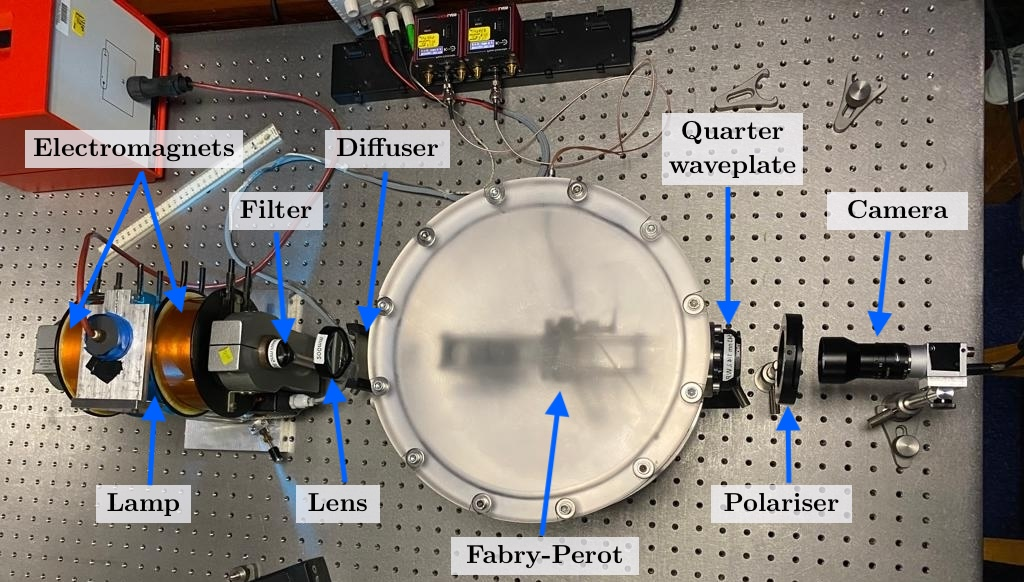
\includegraphics[width=0.65\linewidth]{setup photo.jpeg}
    \captionsetup{justification=centering}
    \caption{Experimental setup in the parallel observation configuration, iris not included. See schematic illustration if Fig. \ref{fig: setup}}
    \label{fig: setup photo}
\end{figure}

\section{Appendix - Current to field conversion}
We cannot measure the magnetic field while having the lamp in position due to space constraints. Therefore we instead measure the magnetic field indirectly, by measuring the current flowing through the electromagnets. This requires a current-field calibration, sown is Figure \ref{fig:IvsB}. We use a linear fit $y = a x + b$, with two free parameters, in order to take into account the possibility of having some residual magnetic field caused by the iron cores becoming magnetised. Same procedure was followed for the full iron cores (Figure \ref{fig:IvsB full}) and hollow iron cores (Figure \ref{fig:IvsB hollow}). The best fit parameters are found by the method of least squares: 
\begin{equation}
	\text{Full iron cores: }
	\hspace {1cm} 
	a = 0.312 \pm 0.004  \text{ } \si{T.A^{-1}} 
	\hspace {1cm} 
	b = 0.013 \pm 0.002 \text{ }  \si{T} 
\end{equation}
\begin{equation}
	\text{Hollow iron cores: }
	\hspace {1cm} 
	a = 0.472 \pm 0.004  \text{ } \si{T.A^{-1}} 
	\hspace {1cm} 
	b = 0.032 \pm 0.003  \text{ } \si{T} 
\end{equation}

\begin{figure}[h!]
  \centering
  \begin{subfigure}{0.48\linewidth}
    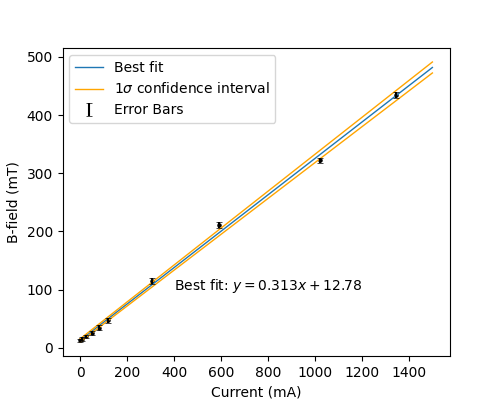
\includegraphics[width=\linewidth]{IvsB full.png}
    \caption{Full iron core}
    \label{fig:IvsB full}
  \end{subfigure}
  \hfill
  \begin{subfigure}{0.48\linewidth}
    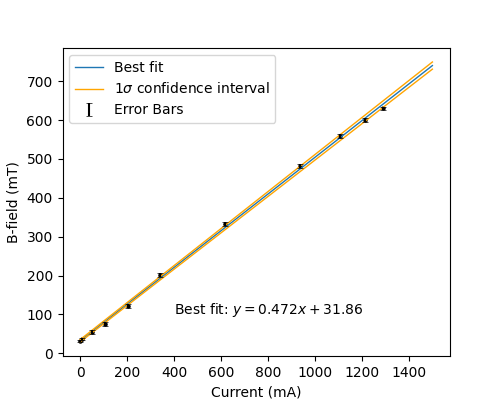
\includegraphics[width=\linewidth]{IvsB hollow.png}
    \caption{Hollow iron core}
    \label{fig:IvsB hollow}
  \end{subfigure}
  \captionsetup{justification=centering}
  \caption{Conversion of the applied current to magnetic field.  The data was fitted with a linear fit ($y = a x + b$) using the method of least squares. Data points shown as central value $\pm$ variation of the field in the gap between the cores. Parameters of the best-fit are: \ref{fig:IvsB full}: $a = 0.312 \pm 0.004 $ \si{T.A^{-1}} and $ b = 0.013 \pm 0.002 $ \si{T} and \ref{fig:IvsB hollow}: $a = 0.472 \pm 0.004 $ \si{T.A^{-1}} and $ b = 0.032 \pm 0.003 $ \si{T}}
  \label{fig:IvsB}
\end{figure}

\section{Appendix - User interface}
The user interface used to make measurements is shown in figure \ref{fig: Cd red}. We used the circle tool to overlay circles on the interference maxima. The circle radius is measured in pixels and then converted to milimiters using the known size of pixels. 

\begin{figure}[h!]
    \centering
    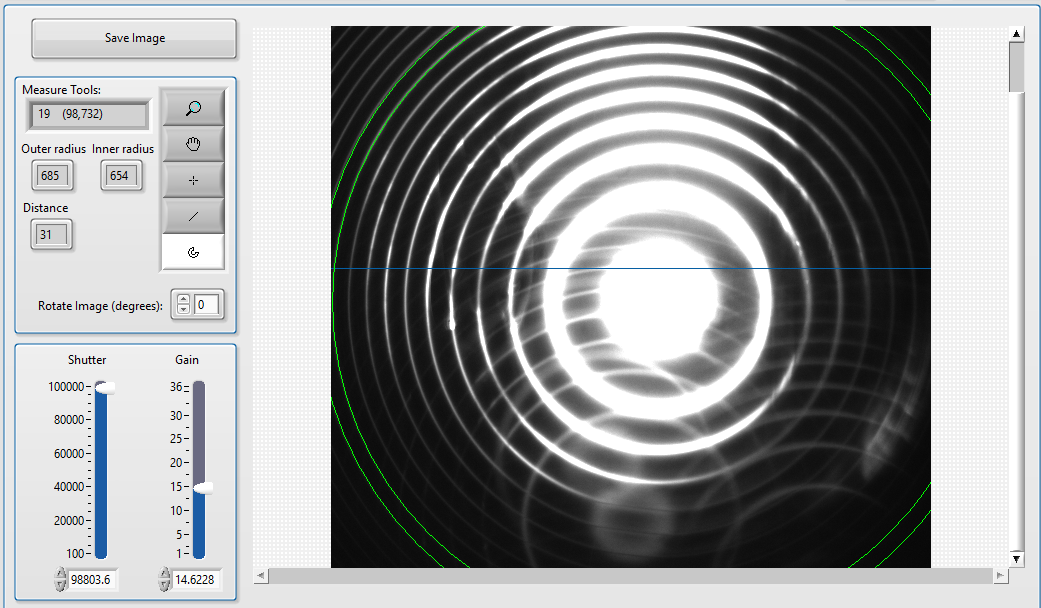
\includegraphics[width=0.65\linewidth]{d measurement.png}
    \captionsetup{justification=centering}
    \caption{User interface of the program used for measurements. Image shows the Fabry-Perot interference pattern of the cadmium red line, no magnetic field applied.}
    \label{fig: d measurement}
\end{figure}

\newpage
%-------------------------------------------------------------------------------------------

\section{Appendix - Splitting measurements plotted}
\subsection{Cadmium}
\begin{figure}[h!]
    \centering
        \begin{subfigure}{\linewidth}
        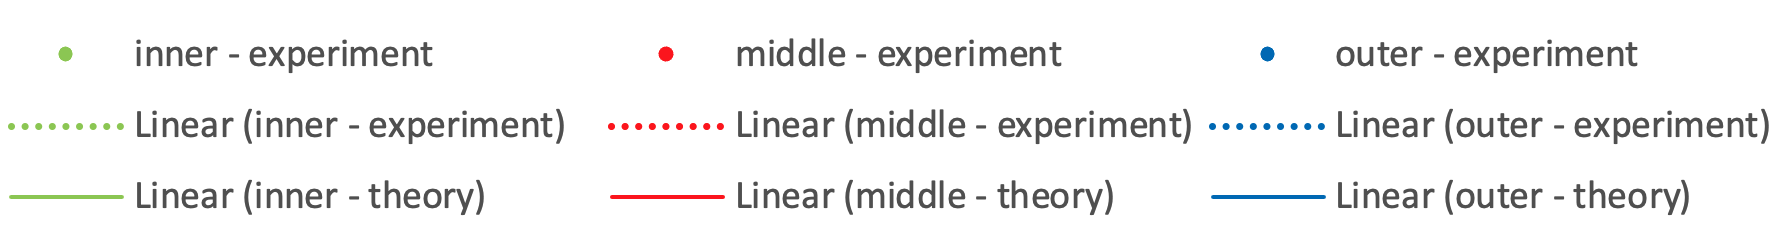
\includegraphics[width=\linewidth]{splitting graphs/legend.png}
    \end{subfigure}
    \begin{subfigure}{0.47\linewidth}
        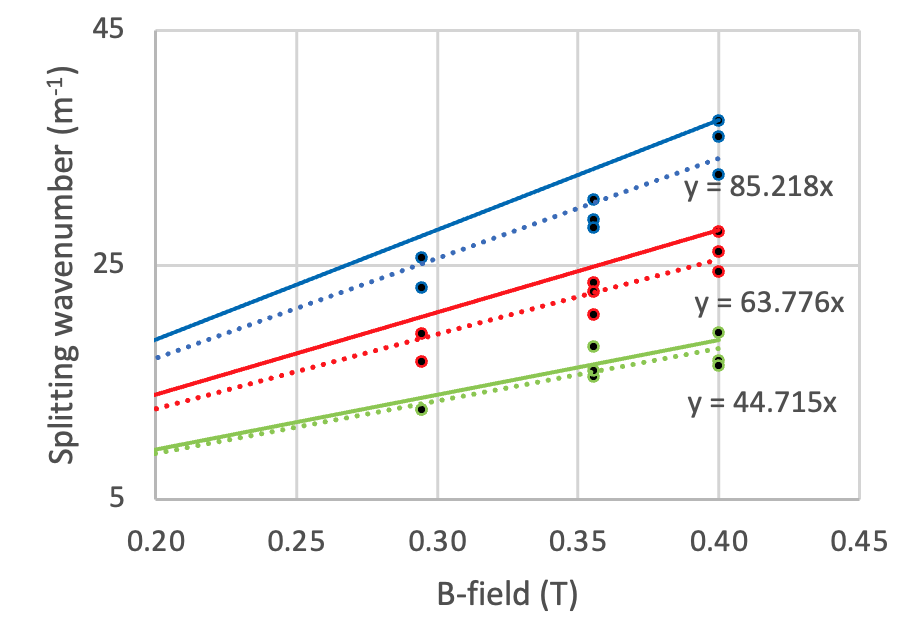
\includegraphics[width=\linewidth]{splitting graphs/Cd green sigma perp gr.png}
        \caption{observation perpendicular to B-field}
        \label{fig: Cd green sig perp}
    \end{subfigure}
    \begin{subfigure}{0.47\linewidth}
        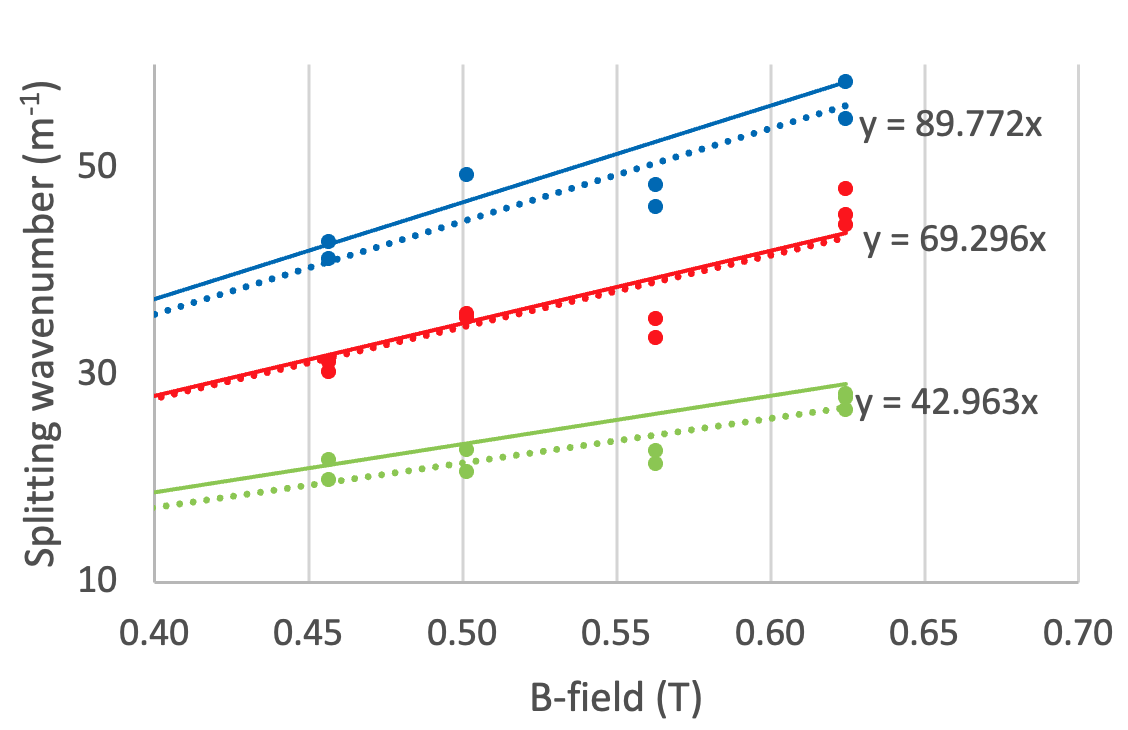
\includegraphics[width=\linewidth]{splitting graphs/Cd green sigma par gr.png}
        \caption{observation parallel to B-field}
        \label{fig: Cd green sig par}
    \end{subfigure}
    \caption{Line splitting due to Zeeman effect in the $\sigma$ polarised lines in the cadmium green line. "inner", "middle" and "outer" data correspond to the pairs of lines labelled (1, 1'), (2, 2') and (3, 3') in Fig. \ref{img: Cd_green_sigma_increasing_field}. We used a linear fit with intercept of 0 to fit the data. Theoretical dependence is shown with a solid line.}
\end{figure}

\begin{figure}[h!]
    \centering
    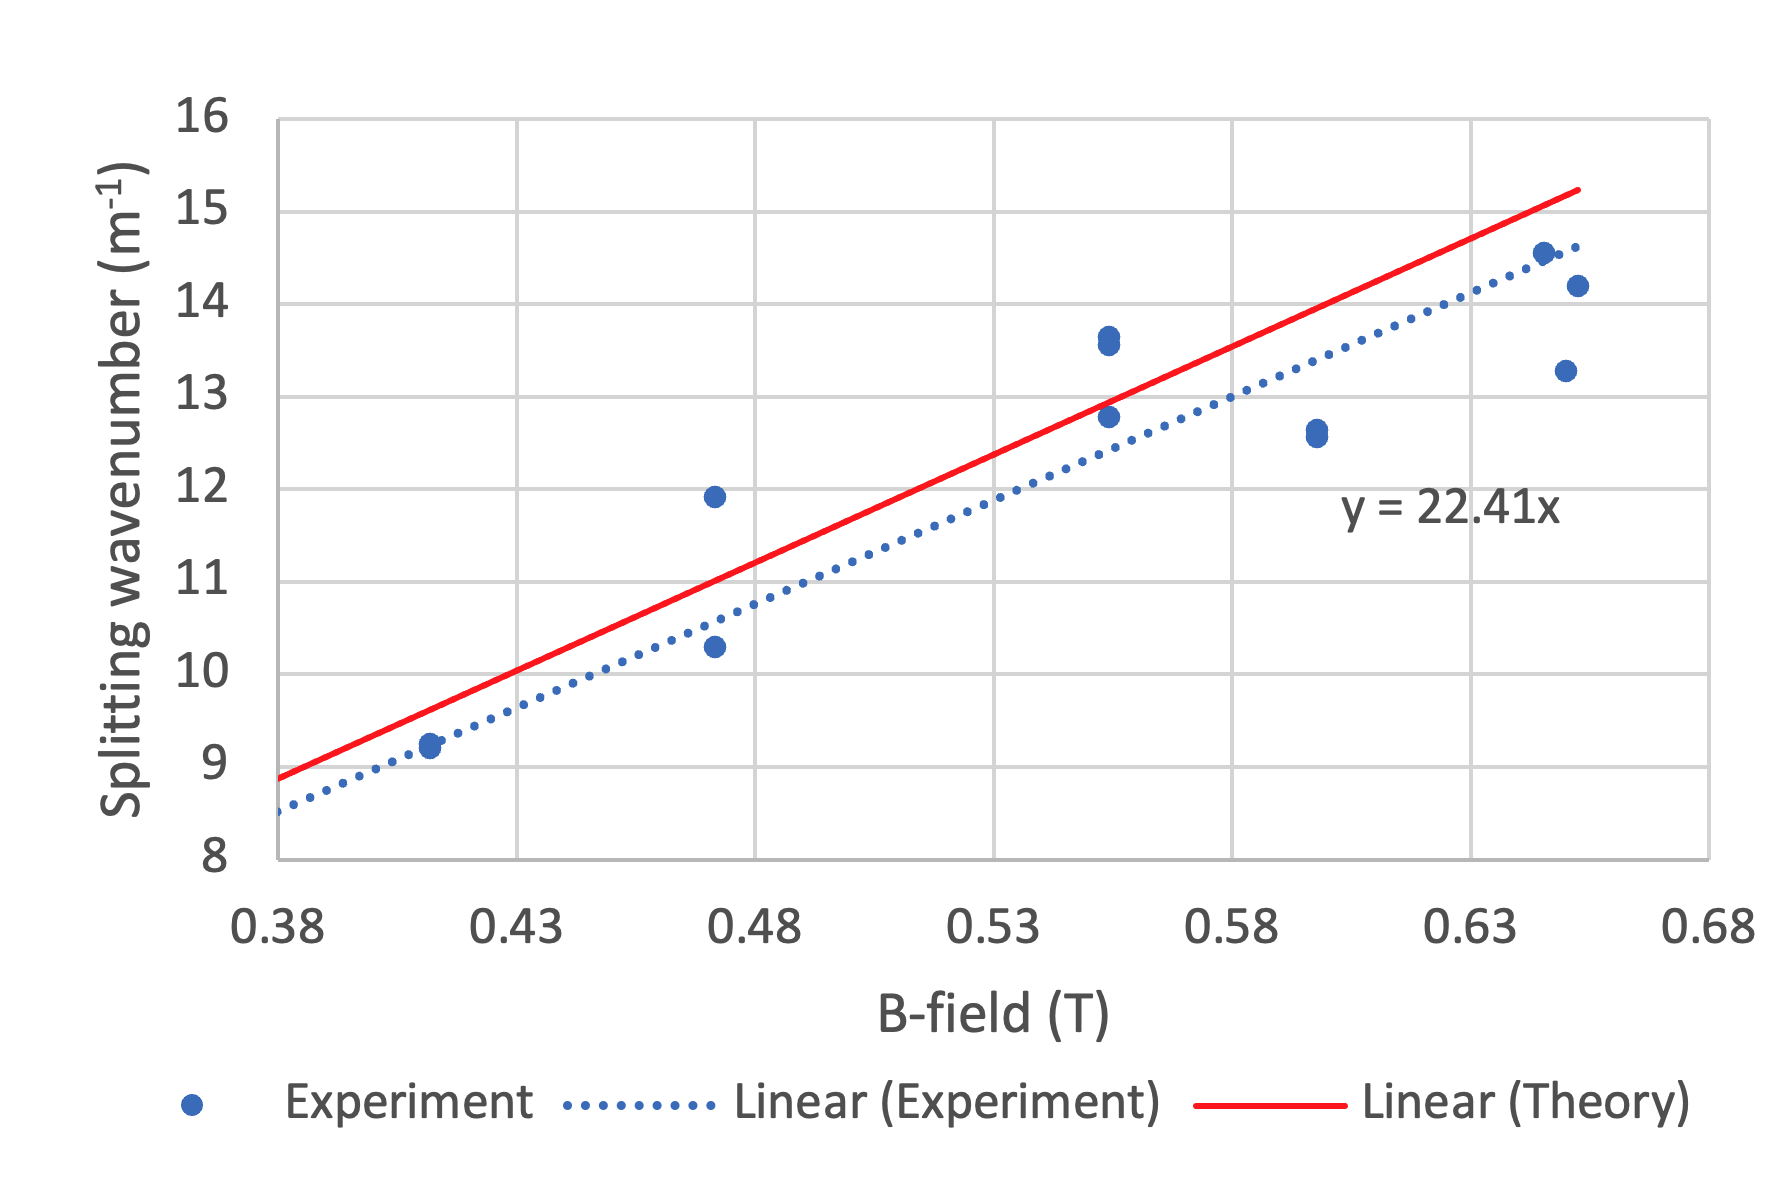
\includegraphics[width=0.7\linewidth]{Cd green pi perp small.png}
    \captionsetup{justification=centering}
    \captionsetup{width=\linewidth}
    \caption{Line splitting due to Zeeman effect in the $\pi$ polarised lines in the cadmium green line with the perpendicular configuration}
    \label{fig: Cd green pi}
\end{figure}

\newpage

\subsection{Mercury}

\begin{figure}[h!]
    \centering
    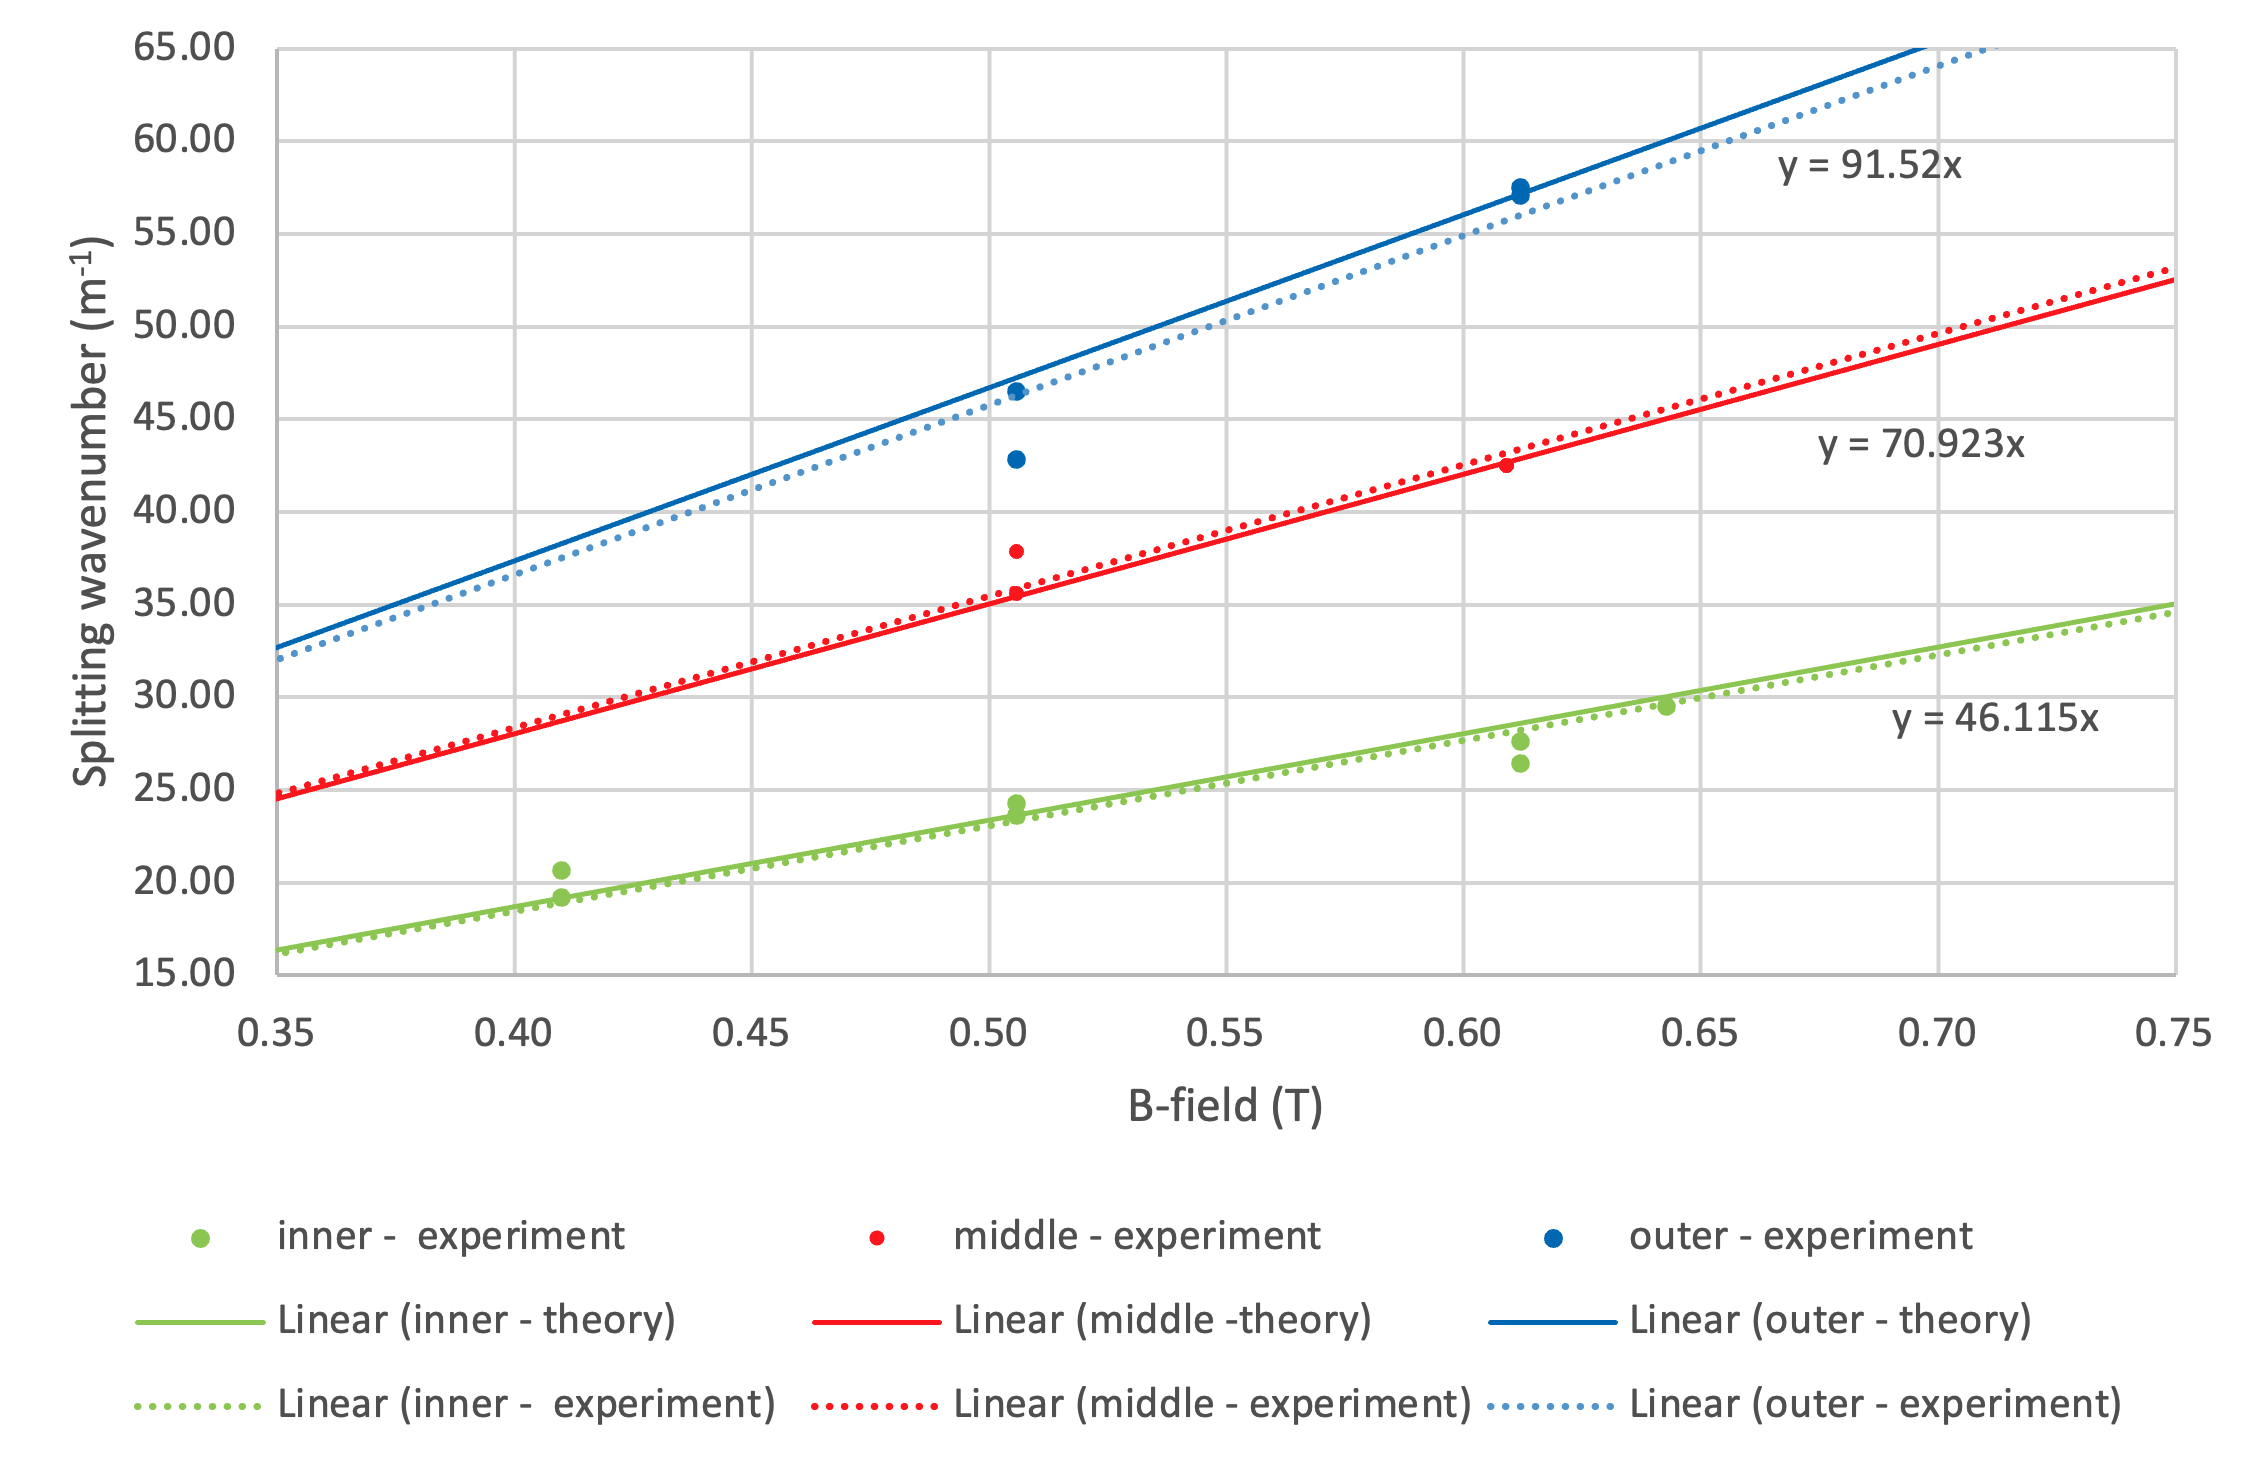
\includegraphics[width=0.9\linewidth]{Hg green sigma par graph.png}
    \captionsetup{width=\linewidth}
    \captionsetup{justification=centering}
    \caption{Line splitting due to Zeeman effect in the $\sigma$ polarised lines in the mercury green line with the parallel configuration. The dotted lines are the linear fits of the measurements, the solid lines are theoretical predictions. Inner, middle and outer components are shown in green, red and blue and correspond to the (1, 1'), (2, 2') and (3, 3') pairs respectively (see Fig. \ref{img: Cd_green_sigma_increasing_field})}
    \label{fig: Hg green sigma}
\end{figure}

\begin{figure}[h!]
\centering
    \begin{minipage}[c]{0.47\textwidth}
        \centering
        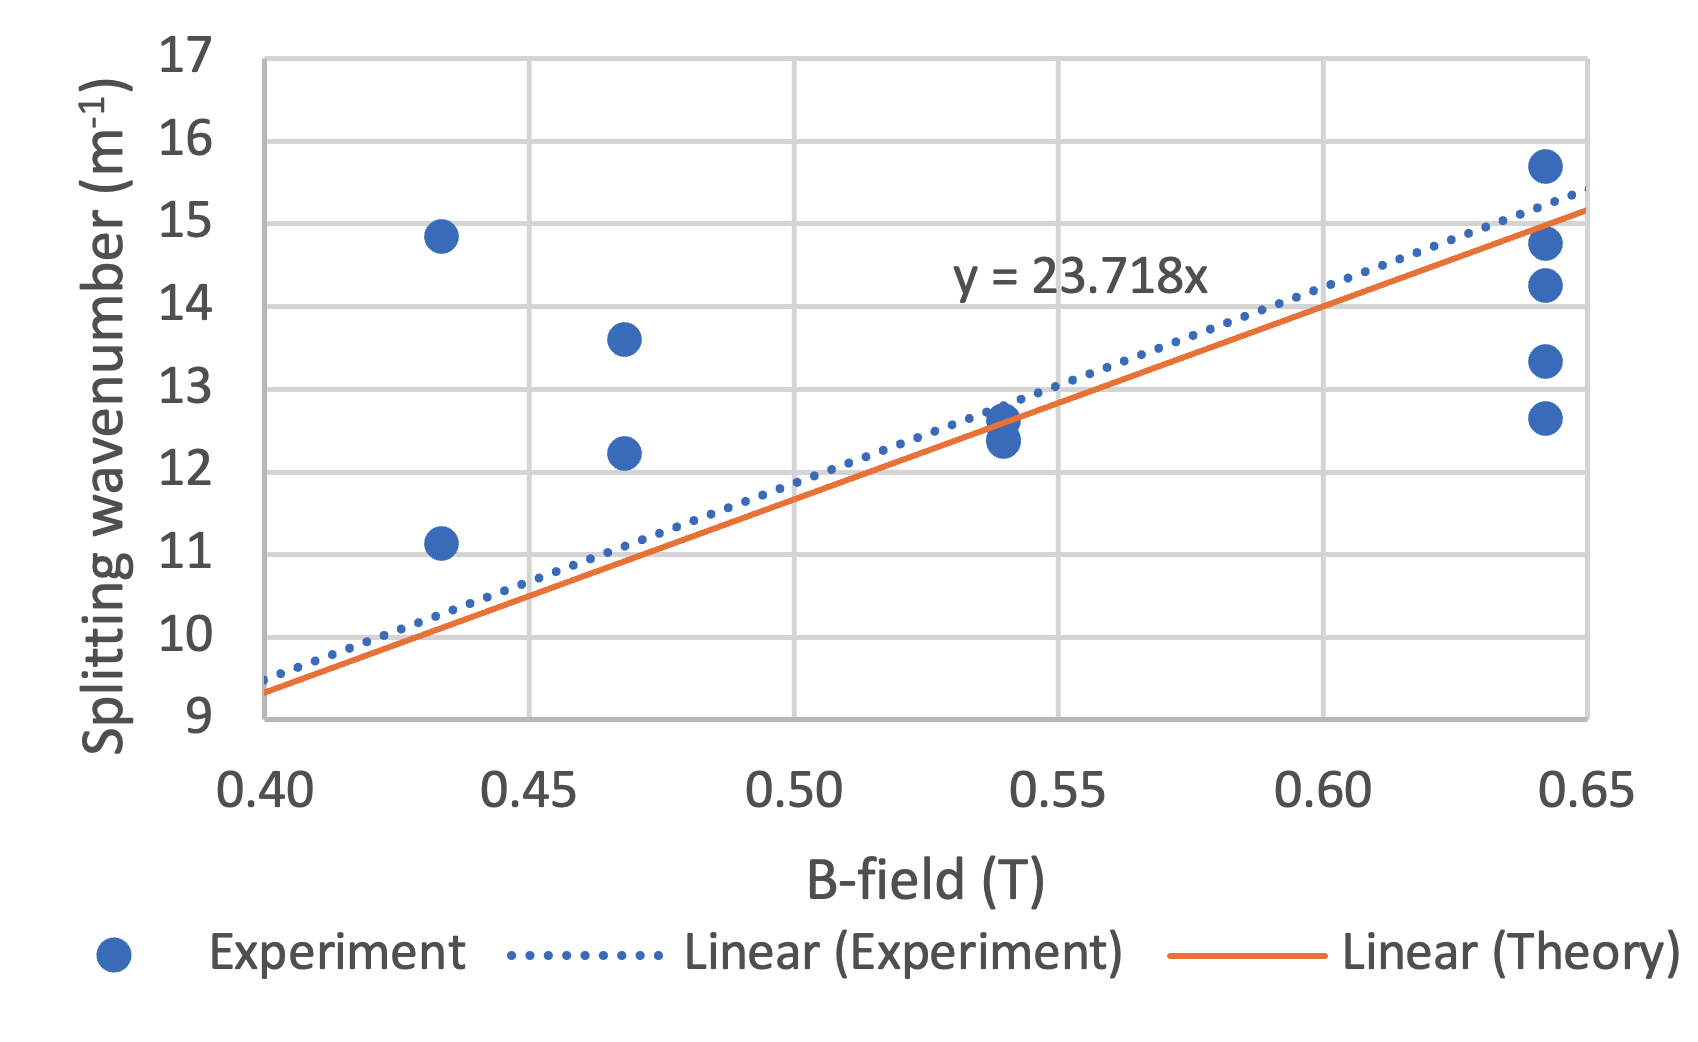
\includegraphics[width=\linewidth]{Hg green pi perp small.png}
        \captionsetup{width=0.9\linewidth}
        \caption{Line splitting due to Zeeman effect in the $\pi$ polarised lines in the mercury green line with the perpendicular configuration}
        \label{fig: Hg green pi}
    \end{minipage}
    \begin{minipage}[c]{0.47\textwidth}
        \centering
        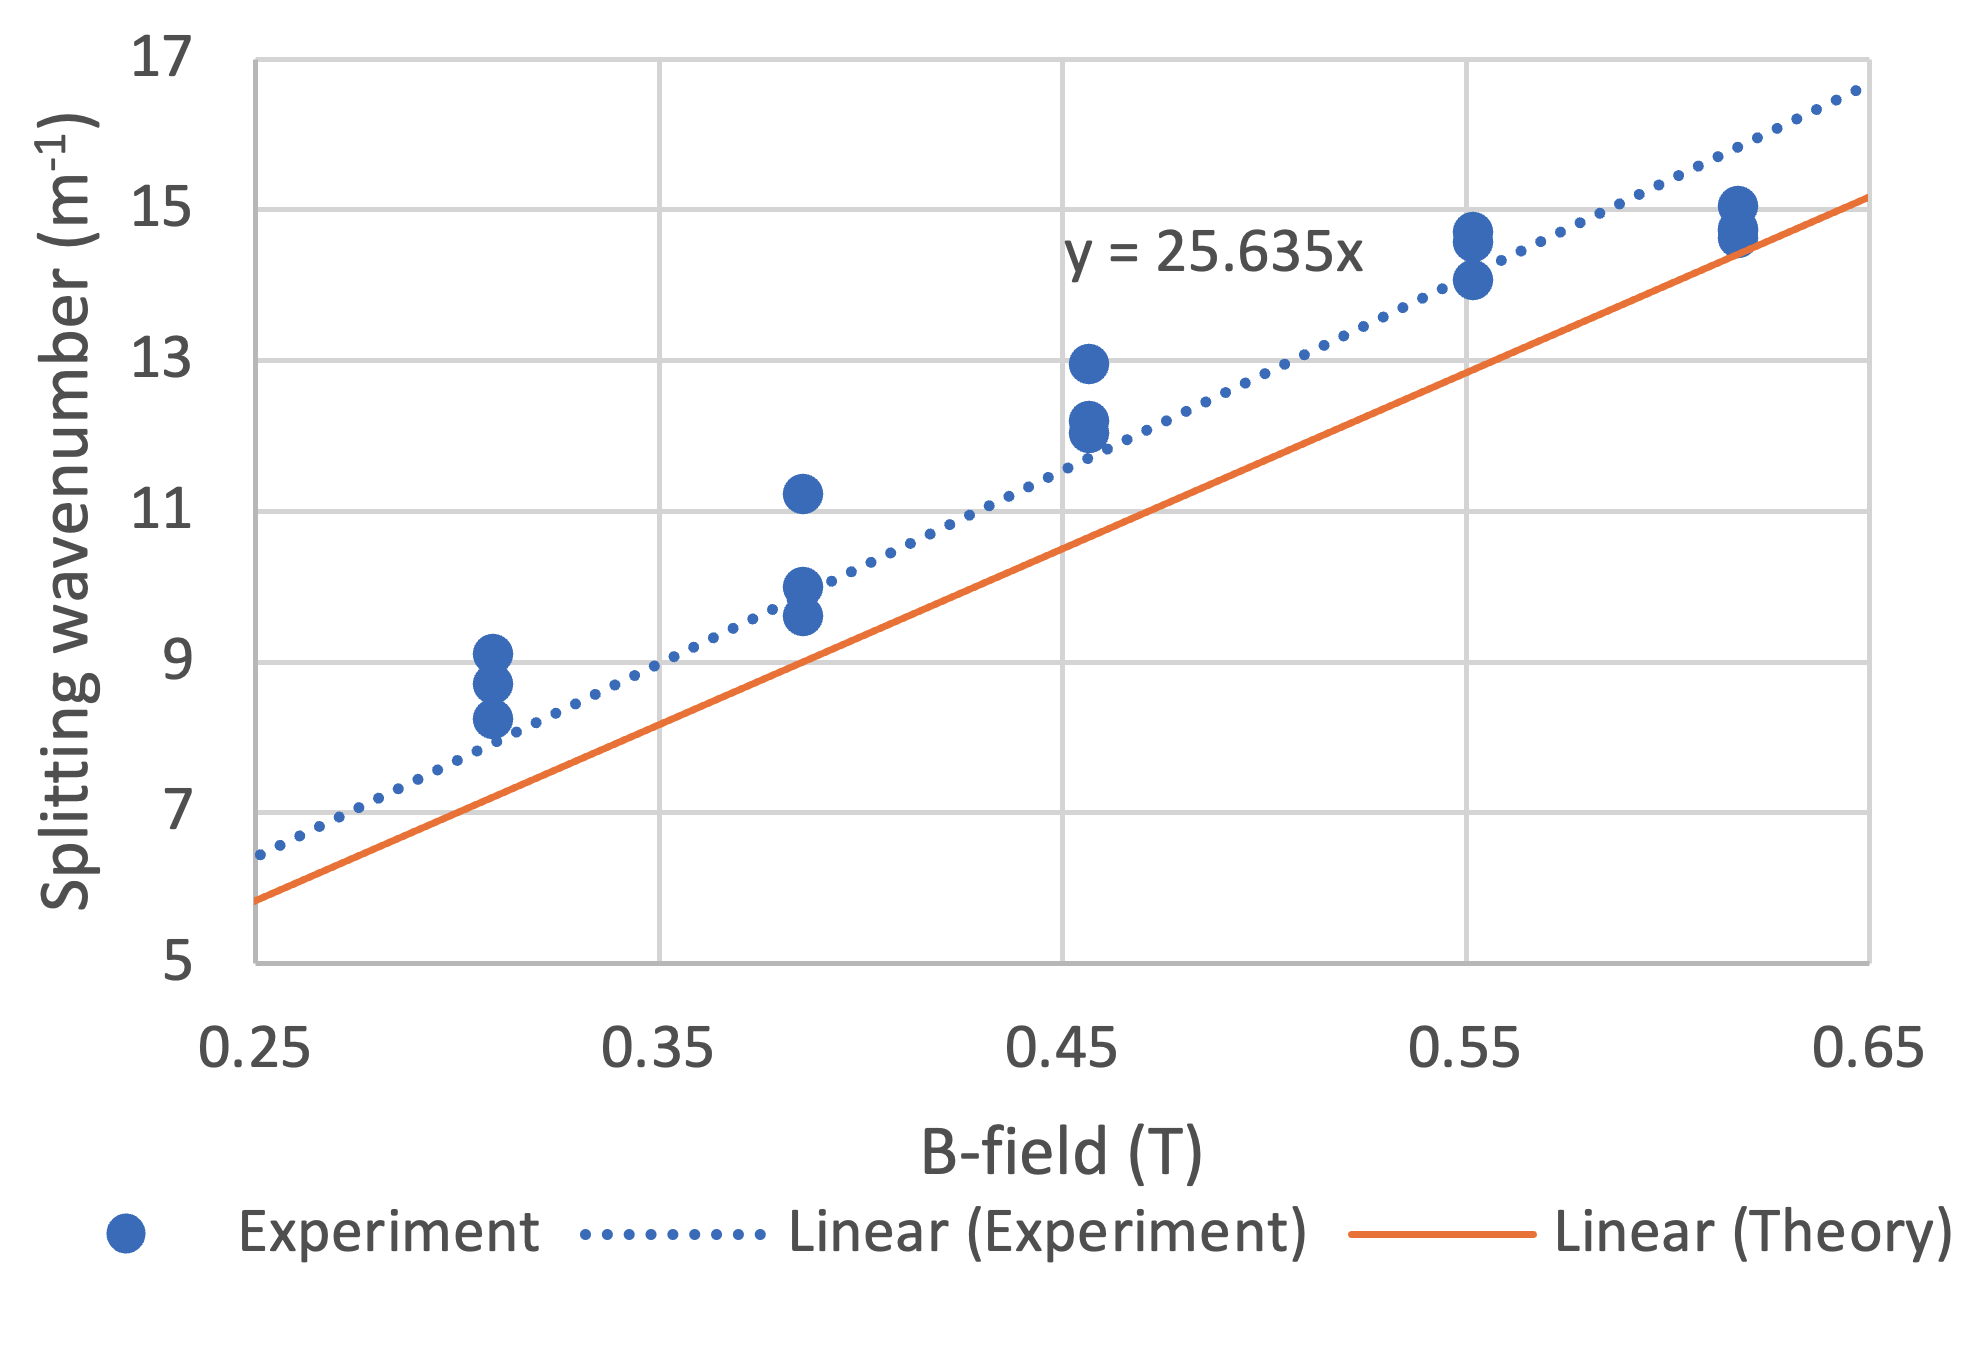
\includegraphics[width=\linewidth]{Hg blue pi perp small.png}
        \captionsetup{width=0.9\linewidth}
        \caption{Line splitting due to Zeeman effect in the $\pi$ polarised lines in the mercury blue line with the perpendicular configuration}
        \label{fig: Hg blue pi}
    \end{minipage}
\end{figure}

\begin{table}[h!]
    \centering
    \begin{tabular}{c|ccc}
    \toprule
         \( g_{eff} \) & B-field $\si{T}$ &  Measured $\Delta \nu \pm \mathrm{FWHM } (\si{m^{-1}})$ & Theoretical $\Delta \nu$ $(\si{m^{-1}})$\\
         \midrule
         $\pm 1.5$& 0.5 & $36.8 \pm 8$ & 35.28 \\
         $\pm 2$ & 0.5 & $44.97 \pm 8$ & 47.04 \\
    \end{tabular}
    \caption{Measurements of the line splitting $\Delta \nu$ in the mercury blue sigma lines}
    \label{tab: Hg blue sigma measurements}
\end{table}

\newpage
\section{Appendix - Camera and Fabry-Perot images}
All the images used for the data analysis and presented in the report are taken with the Basler acA1920-40um camera \footnote{https://docs.baslerweb.com/aca1920-40um} provided by the physics undergraduate practical labs, unless stated otherwise. This camera captures black and white images with 8 bit colour accuracy, resulting in 256 possible pixel brightness values. The camera has a full resolution of 1936 by 1216 pixels, but the custom practical labs software used in the practical labs only makes use of a section of the images of size 1200 by 1200. The images are exported in .png format, also at the 1200 by 1200 resolution. 

The focus and aperture are manual, mechanical settings adjusted by a zoom ring and a focus ring. The aperture of the camera is opened all the way, to maximise the amount of light hitting the sensor, and to minimise diffraction effects. The camera is focused such that the image of the lamp is sharp (with the Fabry-Perot interferometer removed). 
The shutter speed and gain of the camera are adjusted digitally, through the practical lab software. We aim to keep the gain as low as possible, to reduce noise in the image.  

We do not know if the camera has a linear intensity response or not, and we cannot measure this with the instruments available in the lab. In order to characterise the response of the camera we would need a calibrated light source. Since we do not know if the response of the camera is linear, and we don't know how the shutter and gain settings affect the response, it is impractical to try to quantitatively measure the relative intensities of the different components. Nonetheless, the images clearly show that some of the lines observed are brighter than others. 
\begin{figure}[h!]
    \centering
    \begin{minipage}[t]{0.47\linewidth}
        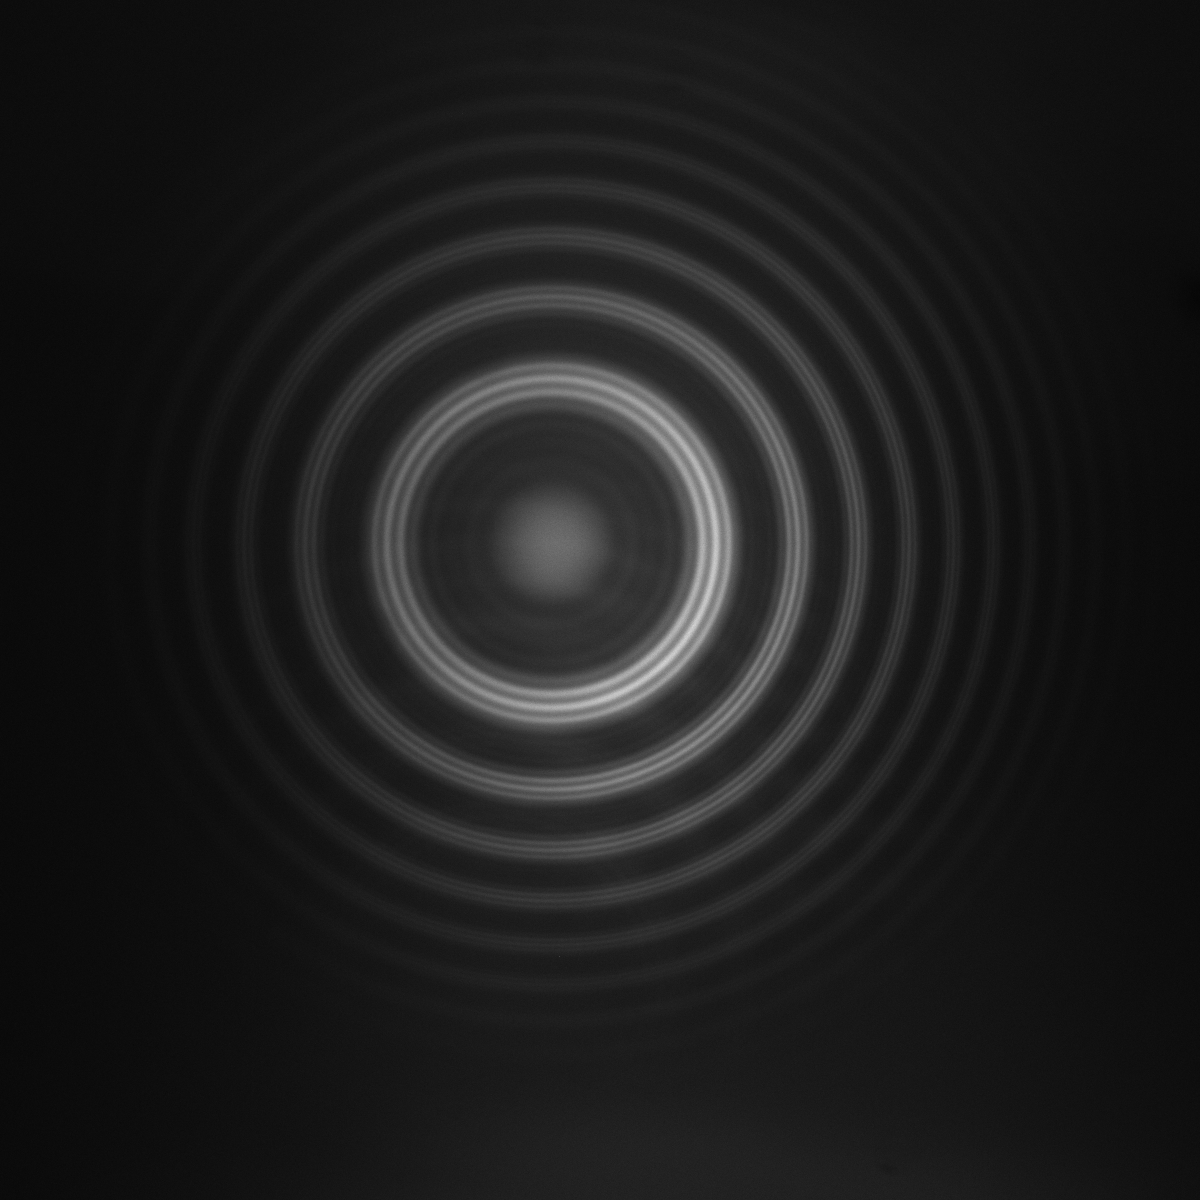
\includegraphics[width=\linewidth]{mr pi green zeeman 2.png}
        \captionsetup{justification=centering}
        \caption{Fabry-Perot interferometer image of the cadmium green line with magnetic field applied in the perpendicular configuration. Only $\pi$ lines visible}
        \label{img: Cd green pi perp}
    \end{minipage}\hfill
    \begin{minipage}[t]{0.47\linewidth}
        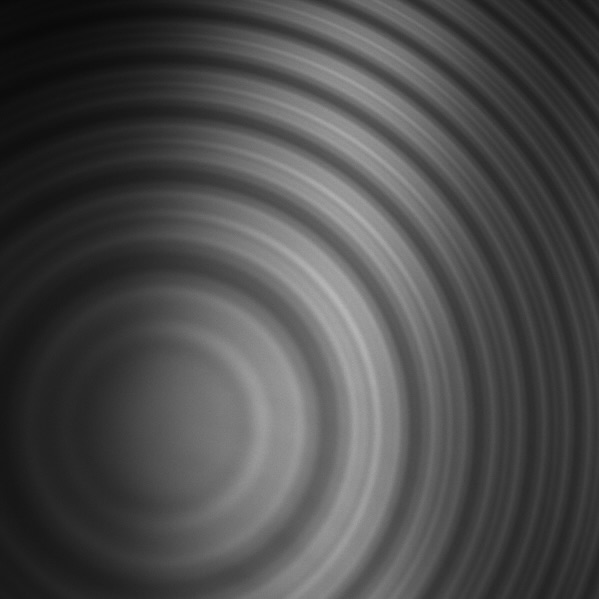
\includegraphics[width=\linewidth]{hg green 9 lines cropped.jpeg}
        \captionsetup{justification=centering}
        \caption{Cropped Fabry-Perot interferometer image of the mercury green line with magnetic field applied in the perpendicular configuration. All 9 split components are visible. The outer components have low relative intensity and the split components fill the full spectral range of the interferometer, therefore it might be hard to identify all components without adjusting the magnetic field. }
    \end{minipage}
\end{figure}
\begin{figure}[h!]
    \centering
    \begin{minipage}[t]{0.47\linewidth}
        \centering
        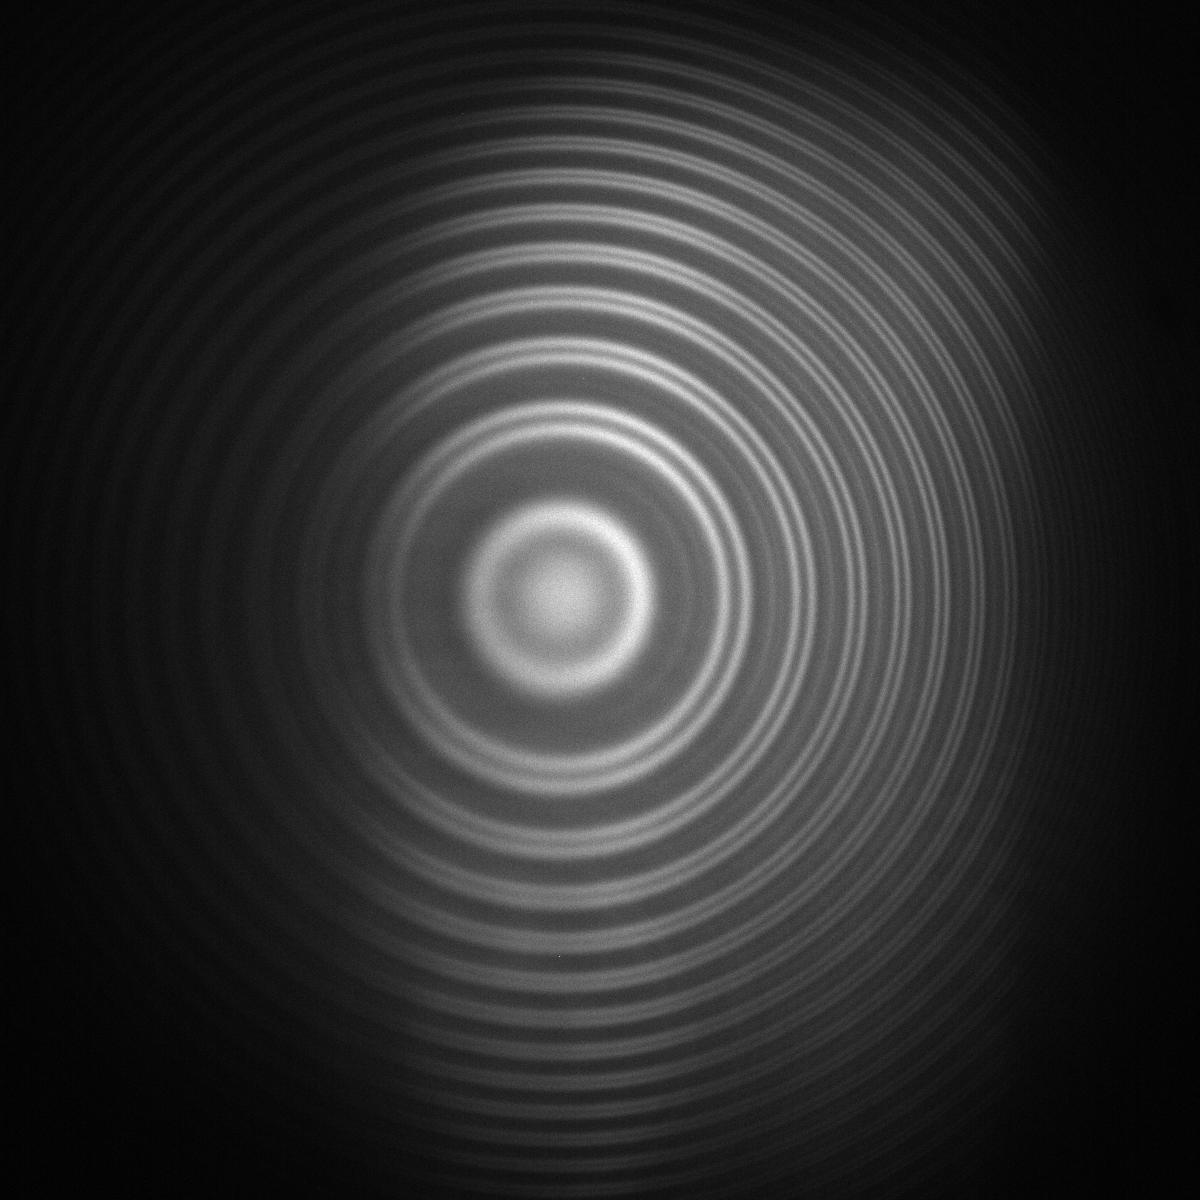
\includegraphics[width=\linewidth]{Hg blue pi high zeeman.png}
        \captionsetup{justification=centering}
        \caption{Fabry-Perot interferometer image of the mercury blue line with magnetic field applied in the perpendicular configuration. Only $\pi$ lines visible}
        \label{img: Hg blue pi perp}
    \end{minipage}\hfill
    \begin{minipage}[t]{0.47\linewidth}
        \centering
        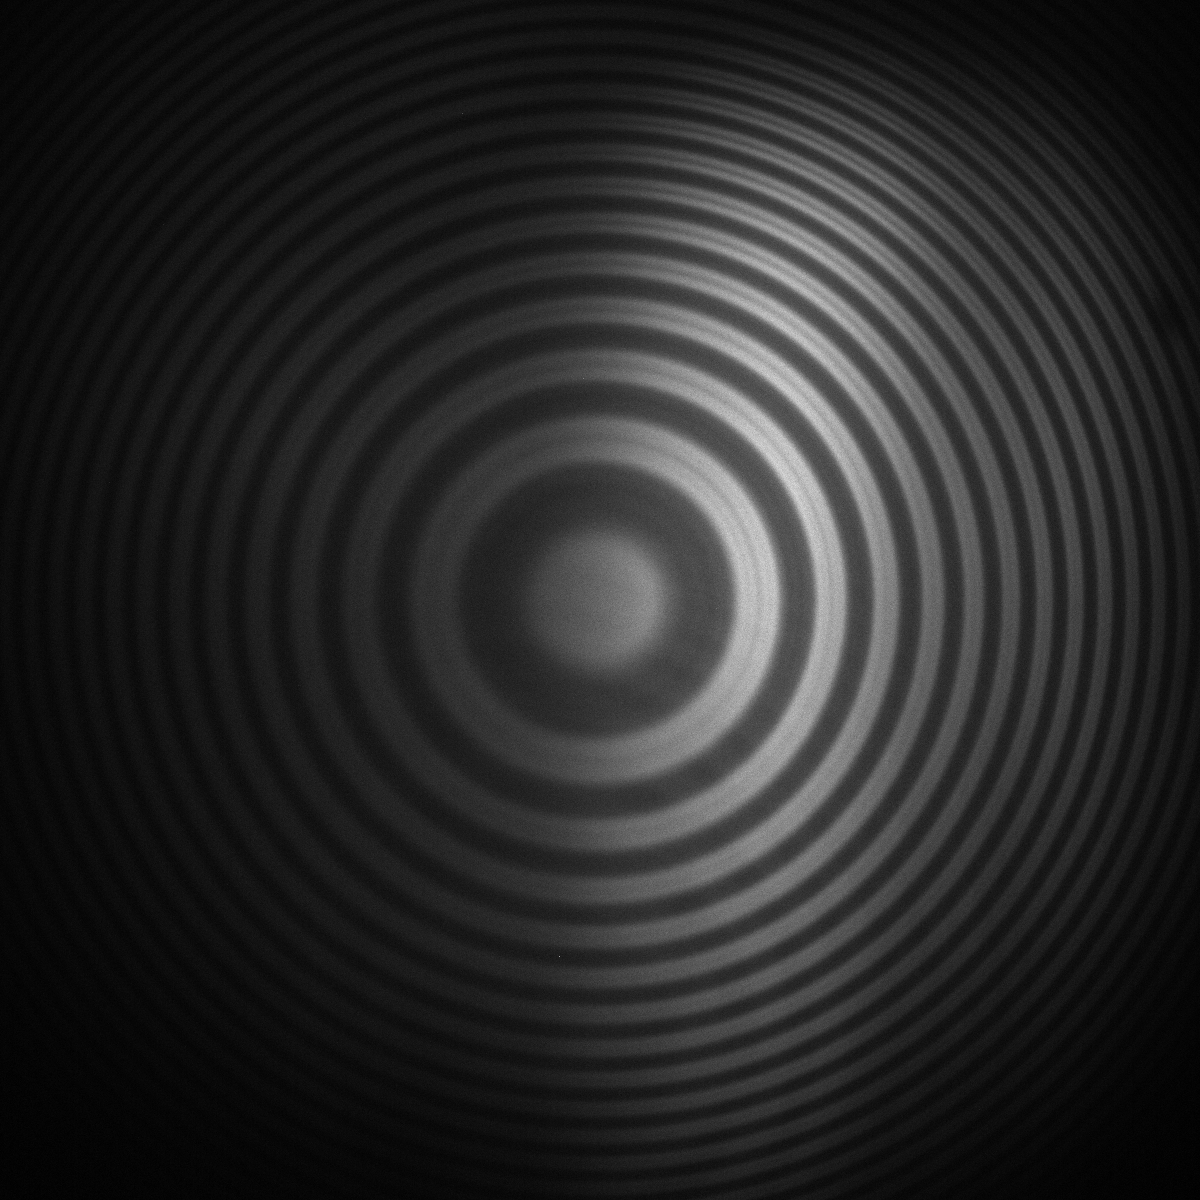
\includegraphics[width=\linewidth]{hg blue sigma lines nearly overlapping.png}
        \captionsetup{justification=centering}
        \caption{Fabry-Perot interferometer image of the mercury blue line with magnetic field applied. Only $\sigma$ lines visible}
        \label{img: Hg blue sigma}
    \end{minipage}
\end{figure}

\newpage

\section{Appendix - Line profiles of the instrument} \label{sec: Line profiles}
The experiment investigated the line profiles of the instrument (section \ref{sec: resolution measurement}) in order to characterise the resolution of the Fabry-Perot interferometer and determine the leading source of uncertainty. Line profiles were plotted using the mercury light (Fig. \ref{img: Hg line profile}) and using a Helium-Neon laser with a much narrower inherent line width. The laser light also had a much narrower beam, reducing the importance of having an interferometer with perfectly flat plates. Both of these facts reduced the FWHM observed (Fig. \ref{img: He-Ne line profile} and \ref{img: He-Ne image}).
\begin{figure}[h!]
    \centering
    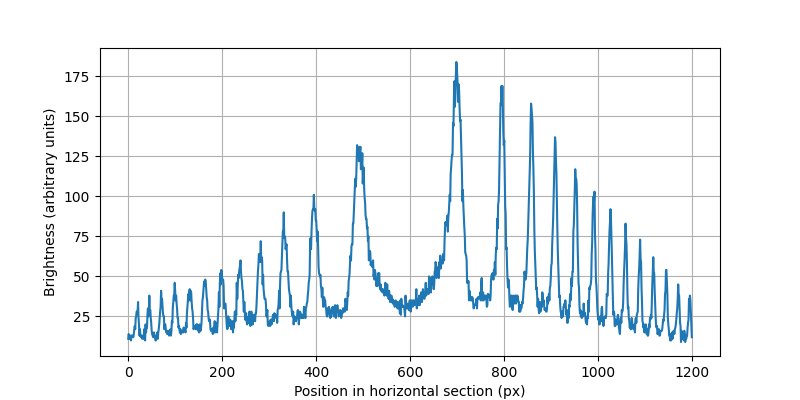
\includegraphics[width=\linewidth]{line profiles/Hg line profile no field 2.png}
    \captionsetup{justification=centering}
    \caption{Horizontal line profile through the centre of the Fabry-Perot interference pattern produced by the mercury blue line with no external magnetic field applied}
    \label{img: Hg line profile}
\end{figure}
\begin{figure}[h!]
    \centering
    \begin{minipage}[c]{0.67\textwidth}
        \centering
        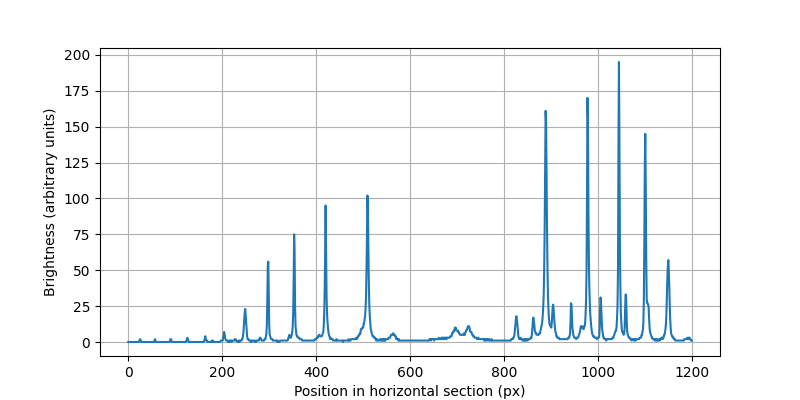
\includegraphics[width=\linewidth]{line profiles/HeNe laser.png}
        \captionsetup{justification=centering}
        \caption{Horizontal line profile through the centre \\
        of the Fabry-Perot interference pattern produced \\
        by the He-Ne laser}
        \label{img: He-Ne line profile}
    \end{minipage}
    \begin{minipage}[c]{0.3\textwidth}
        \centering
        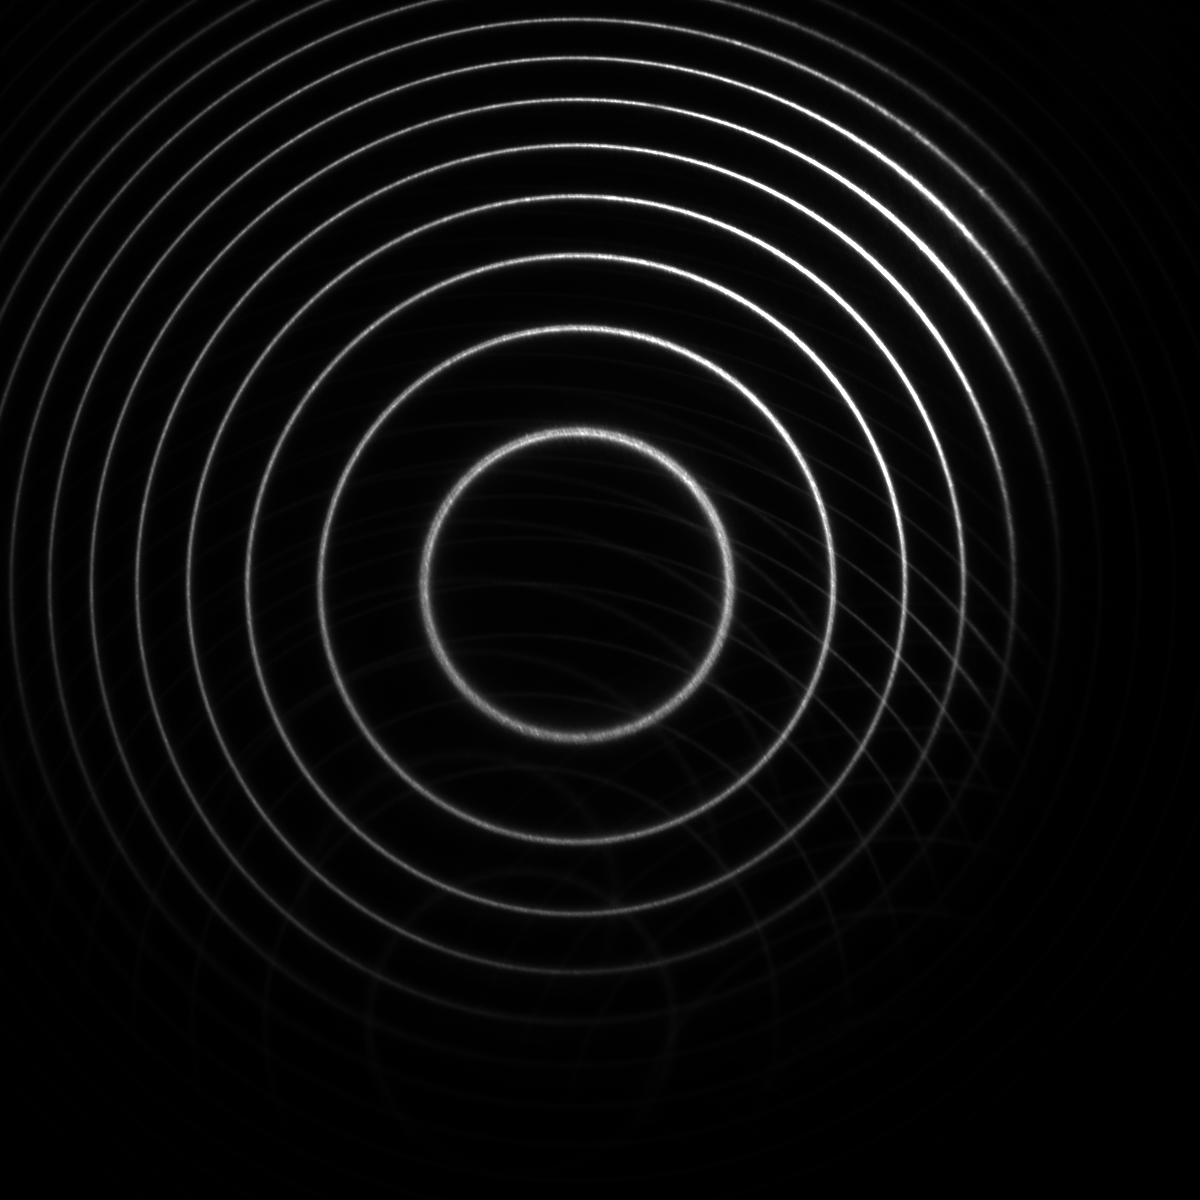
\includegraphics[width=\linewidth]{line profiles/helium neon laser (paper smooted).png}
        \captionsetup{justification=centering}
        \caption{Fabry-Perot interference pattern produced by the He-Ne laser}
        \label{img: He-Ne image}
    \end{minipage} 
\end{figure}

\end{document}